\documentclass[12pt]{article}
\usepackage{amsmath}
\usepackage{graphicx,psfrag,epsf}
\usepackage{enumerate}
\usepackage{natbib}
\usepackage{url} % not crucial - just used below for the URL 
\usepackage{tabularx}
%\pdfminorversion=4
% NOTE: To produce blinded version, replace "0" with "1" below.
\newcommand{\blind}{0}

% DON'T change margins - should be 1 inch all around.
\addtolength{\oddsidemargin}{-.5in}%
\addtolength{\evensidemargin}{-.5in}%
\addtolength{\textwidth}{1in}%
\addtolength{\textheight}{-.3in}%
\addtolength{\topmargin}{-.8in}%

\usepackage{amsmath,amssymb,amsthm,amsfonts,amstext,amsbsy,amscd,stmaryrd}
\usepackage{amssymb,amsmath,comment,subcaption,graphicx}
\usepackage{multirow}
\usepackage{multicol}
\usepackage{algorithm}
\usepackage{algorithmic}
\usepackage{cancel}
\usepackage{tikz}
\usepackage{subcaption}
\usetikzlibrary{patterns}
\usepackage{xcolor}
\usepackage{bbm}
\usepackage{float}
\usepackage{color}
\usepackage{relsize}
\newcommand{\modif}[1]{{\begin{modification}#1\end{modification}}}
\newcommand{\ele}[1]{{\color{red}#1}}
%\UseRawInputEncoding
\DeclareMathOperator*{\argmax}{arg\,max}
\DeclareMathOperator*{\argmin}{arg\,min}
\usepackage{mathrsfs}
\newcommand{\rmd}{{\mathrm{d}}}
\newcommand{\R}{\mathbb{R}}
\newcommand{\N}{\mathbb{N}}
\newcommand{\PP}{\mathbb{P}}
\newcommand{\V}{\mathbb{V}}
\newcommand{\Z}{\mathbb{Z}}
\renewcommand{\P}{\mathbb{P}}
\newcommand{\E}{\operatorname{\mathbb{E}}}
\newcommand{\Var}{\operatorname{Var}}
\newcommand{\Cov}{\mathrm {Cov}}
\newcommand{\rme}{{\rm e}}
\renewcommand{\tilde}{\widetilde}
\renewcommand{\hat}{\widehat}
\newcommand{\TC}{\mathrm{TC}}
\newcommand{\TaC}{\mathrm{TaC}}
\newcommand{\LTC}{\mathrm{LTC}}
\newcommand{\LP}{\mathrm{LP}}
\newcommand{\Per}{\mathrm{Per}}
\theoremstyle{Theorem}
\newtheorem{Theorem}{Theorem}[section]
\newtheorem{Corollary}[Theorem]{Corollary}
\newtheorem{Lemma}[Theorem]{Lemma}
\newtheorem{Proposition}[Theorem]{Proposition}
\newtheorem{Definition}[Theorem]{Definition}
\newtheorem{remark}{Remark}
\renewcommand{\labelitemi}{\textperiodcentered}
\allowdisplaybreaks
\usepackage{ifpdf}
\ifpdf
\else
\usepackage{graphicx}
\DeclareGraphicsExtensions{.eps,.jpg,.png}
\fi
\usepackage{epstopdf}

\newcommand{\overbar}[1]{\mkern 1.5mu\overline{\mkern-1.5mu#1\mkern-1.5mu}\mkern 1.5mu}
\newcolumntype{Y}{>{\centering\arraybackslash}X}

\parindent 0mm    
\RequirePackage[colorlinks,citecolor=blue,urlcolor=blue]{hyperref}
\tikzset{
    cross/.pic = {
    \draw[rotate = 45] (-#1,0) -- (#1,0);
    \draw[rotate = 45] (0,-#1) -- (0, #1);
    }
}

\tikzset{
  mycross/.pic={
    \draw[pic actions] 
      (-2pt,0) -- (2pt,0)
      (0,-2pt) -- (0,2pt);
  },
}

\begin{document}
\section{Introduction}
\textbf{Cabana : Affine Processes: A test of isotropy based on level sets.} 
Class of affine processes for the alternative, $H_{0} :X$ is isotropic, create the test using Estimators for the affinity parameters based only on one level set of the observed process, show consistence under some hypothesis. Proposes estimators of the affinity parameters $k = (1 - \frac{\lambda_{1}^{2}}{\lambda_{1}^{2}})$ and $\theta_{0}$ using the shape of the level curve of $X$ for fixed level $x$. Gets TCL for estimators under condition of \textit{X is uniformly mixing}. \\
Let $\mathscr{C}$ is the level sets, principal objects that are used are $\mathscr{L}(T) = |T|^{-1}\int_{\mathscr{C}}ds$, $\mathscr{C}(T) = |T|^{-1}\int_{\mathcal{C}} \cos\Theta ds$, $\mathscr{S}(T) = |T|^{-1}\int_{\mathscr{C}} \sin2\Theta ds$ that are particular c*ases of line integrals : $\mathscr{F}(f, T) = |T|^{-1}\int_{\mathscr{C}}f(\Theta)ds$, with $f:(-\pi, \pi) \to \mathbb{R}$ is a bounded measurable function.\\
Weird assumptions imply that integrals such as $\mathscr{F}$ have a first and second moment. When we assume that the field $X(t) = Y(At)$ with $Y$ isotropic and we substitute $f$ with the function that are of interest for us, we get a formula for the first moment of $\mathscr{L}$, $\mathscr{C}$ and $\mathscr{S}$. that only depends on $\lambda_{1}, k$ and $\theta_{0}$ and a weird function $g$ that is a continuously increasing function. Thus, we get that $\tan 2\theta_{0} = E\mathscr{S}/E\mathscr{C}$ and $g(k) = \sqrt{(E\mathscr{C})^2 + (E\mathscr{S})^2}/E\mathscr{L}$, \textbf{Asymptotic distributions}. Assuming the field $X$ is uniformly mixing, then we have a TCL for $\mathscr{F}(f, T)$ when the window goes to infinity, that give them the fact that $\hat{\theta_{0}}$ and $\hat{k}$ are consistent. $k$ measures the departure from isotropy. I didn't understand the last paragraph of page 5. But something leads them to consider an $F$ test of isotropy. Considering a horrible test variable $\mathscr{B}(\mathscr{T})$ with $\mathscr{T}$ is partition of $T$, they know that its distribution under $H_{0}$ ($k = 0$) tends to $F_{2, 2n-2}$ $n$ the number of partitions, if $X$ is an affine process, but not isotropic ($k \neq 0$) than the limit law is a non central F, as it is apparently well known from the analysis of variance. The critical region $\mathscr{B}(\lambda \mathscr{T}) > F_{2, 2n-2}(1-\alpha)$ ($\lambda \to \infty$ is an expansion parameter). \\
\textbf{Molina and al. : A method for testing anisotropy and quantifying its direction in digital images.}\\
 \textit{The identification of appropriate spatial models require the previous knowledge of the process exploratory properties such as the existence of a directional component which determines an anisotropic behavior of the phenomenon. Techniques used for analyzing anistropy are limited (compared to techniques for exploring stationarity) and they are only devoted to examining "by eye" experimental variograms in
different directions. (I do not know if that is true or not).} \\
They try to detect anisothropy using a method based on second order bi variate \textit{circular statistics} this allows them also to quantify the direction in which it appears. They also present an application of the method to  the flow of seawater through the Strait of Gibraltar. Tools : a parametric procedure based on the calculation of standard and confidence ellipses, well how do they do that ? and what is that. Well, It's pretty weird, they start by considering a sub image $Z_{l,l}$ of the image $Z$ and $Z(s)$ the random variable (yep nothing more on this mystery variable ), from $Z_{l,l}$ they draw $N=\{z_{1}, \ldots, z_{m}\}$ a random sample of $m$ elements, nothing is being said about this random sample. $\overrightarrow{z_{i}z_{j}}$ represents a variation of $Z(s)$ with intensity $|z_{j} - z_{i}|$ in the direction $\gamma$, being 
\begin{equation*}
\gamma = \begin{cases} \arctan{\frac{z_{jy} - z_{iy}}{z_{jx} - z_{ix}}}& \text{if} (z_{j} - z_{i}) > 0, \\
0 & \text{if} (z_{j} - z_{i}) = 0, \\
 \arctan{\frac{z_{jy} - z_{iy}}{z_{jx} - z_{ix}}} + \pi & \text{if} (z_{j} - z_{i})  < 0, 
\end{cases}
\end{equation*}
where $(z_{ix}, z_{iy})$ are the coordinates of intensity $z_i$, same for the other one. Taking the vectors $\overrightarrow{z_{i}z_{j}}$ we obtain the set $\Gamma = \{\gamma_{i}, i = 1, \ldots, n, n = \binom{m}{2}\}$, that contains the orientations in the plane of vectors. Then, they proceed to the computation of the mean vector $\hat{m}$. Given a sample $\Gamma$ its mean vector $\hat{m}$ (of length $r$ and mean angle $\hat{\Phi}$) is calculated as follows : 
\begin{equation*}
\hat{x} = \frac{1}{n} \sum_{i}^{n} b_{i}\cos{\gamma_{i}}, \; \hspace{3cm}  \; \hat{y} = \frac{1}{n}\sum_{i}^{n}b_{i}\sin{\gamma_{i}}
\end{equation*}
\begin{equation*}
r=\sqrt{\hat{x}^{2} + \hat{y}^{2}}, \; \hspace{1cm} \; \hat{\Phi} = \begin{cases} \arctan{\frac{\hat{y}}{\hat{x}}} \hspace{0.5cm} \text{if} \; \hat{x} > 0 , \\
180 + \arctan{\frac{\hat{y}}{\hat{x}}} \hspace{0.5cm} \text{if} \; \hat{x} < 0 
\end{cases}
\end{equation*}
% where $b_{i} = \begin{cases}0 \; \text{if} \; \gamma = 0 \\ 1 \; \text{else} \end{cases}$, for each sample $\Gamma_{1}, \ldots, \Gamma_{d}$ they determine a mean vector of length $r$ and mean angle $\hat{\Phi}$, (They just sample from the same image $Z_{l,l}$...). They use the standard ellipse to analyses these statistics. Hum this is what they say about this \textit{The tips of the vectors of a second order
% sample form a scatter diagram of data with
% standard deviations in the $X$ and $Y$ directions and a
% certain trend upward or downward. The standard ellipse
% describes this behavior in a condensed way: assuming
% normality, roughly $40\%$ of data points fall inside the
% ellipse and $60\%$ of them outside. The parent population
% does not need to be normal, although it is desirable that
% it does not deviate from normality too much.}
% They define the standard ellipse in the following way
% \begin{itemize}
%   \item its center $(\hat{x}, \hat{y})$ \\
%   \item Construct a rectangle with center at $(\hat{x}, \hat{y})$ and sides parallel to the $X$ and $Y$ axes.. 
%   \item the standard ellipse is embedded in the rectangle above (see the article for more details on the construction). 
  % \end{itemize}
By using standard ellipse, they can compute the direction of maximum variability in a direction of angle $\theta$. So, they are able to describe the spatial behavior of the mean vectors, quantifying by the calculation of $\theta$ the direction of maximum variability

\section{Mathematical framework}\label{section1}
\subsection{Construction of the binary image}\label{construction}
\paragraph{Square tiling}
Let $m$ be an integer with $m \geq 2$. Without loss of generality, we consider our observation window as the unit square $S = [0,m]^{2}$ and  we divide our window into $m^{2}$ pairwise disjoint squares. We denote by $G_{m} := \text{\larger[1]{$[$}}0, m \text{\larger[1]{$)$}}^{2} \cap \mathbb{Z}^{2} $ and for $x \in G_{m}$, we define $C_{m}(x)$ as
\begin{equation*}
C_{m}(x) \, := \,x + \text{\larger[1]{$[$}}0, 1 \text{\larger[1]{$]$}}^{2} \subset S.
\end{equation*}
The $C_{m}(x)$ will be referred to as \textit{cells}, to ease up the notations we denote by $x = (x_1, x_2)$ with $x_1, x_2 \in \{0,\ldots, m-1\}$ and $e_1$, $e_{2}$ the element of the canonical base of $\mathbb{R}^{2}$.
We denote by $\mathbb{E}^{(1)}_{m}, \; \mathbb{E}^{(2)}_{m} $ the set of vertical and horizontal edges in $\mathring{S} = (0,m)^{2}$, and $\mathbb{E}_{m} = \mathbb{E}^{(1)}_{m} \cup \mathbb{E}^{(2)}_{m}$ each $w \in \mathbb{E}_{m}$ is a segment of length $1$.
Figure \ref{fig1} shows an example of a square tiling with $m = 4$.
\begin{figure}[h]
\begin{center}
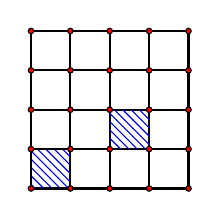
\begin{tikzpicture}[scale = 0.5]
  \draw[step = 1cm, black, thick](0,0) grid (4,4);
\draw[pattern=north west lines, pattern color=blue] (0,0) rectangle (1,1);
\draw[pattern=north west lines, pattern color=blue] (3,1) rectangle (2,2);
\foreach \x in {0,1,2,3,4}{
  \foreach \y in {0,1,2,3,4}{
  \draw[fill = red] (\x,\y) circle (2pt);
  } 
}
\end{tikzpicture}
\end{center}
\vspace{-0.25cm}
\caption{Tiling with squares for $m = 4$ and associated cells $C_{4}(0,0)$ and $C_{4}(2,1)$ (blue stripes) and red point of $G_{m}$.}
\label{fig1}
\end{figure}

\paragraph{Discrete setting}
Using the previous square tiling, we write $S =  \underset{x \in G_m}{\cup}  C_{m}(x)$. We assume to observe $\left(X_{\scriptscriptstyle x}\right)_{x \in G_{m}}$, which we assume coincides with values of a stationary random field $\left(X_{\scriptscriptstyle x}\right)_{x \in \mathbb{Z}^{2}}$. The stationarity hypothesis means that for all $h \in \mathbb{Z}^{2}$, 
$$\left(X_{x+h}; x \in \mathbb{Z}^{2} \right)\overset{fdd}{=} \left(X_{\scriptscriptstyle x}; x \in \mathbb{Z}^{2} \right),$$ where $fdd$ denotes finite-dimensional distributions. \\
We denote by $\rho(x) :=\text{Cov}\left(X_{\scriptscriptstyle 0}, X_{\scriptscriptstyle x}\right), \; x \in \mathbb{Z}^{2}$, the covariance function of $X$.
\vspace{-1.5cm}
\begin{figure}[H]
    {\includegraphics[scale=0.25]{GaussianUn.pdf}}
    {\includegraphics[scale=0.25]{GaussianZUn.pdf}}
    {\includegraphics[scale=0.25]{GaussianZZZUn.pdf}}
    \vspace{-2cm}
 \caption{Generations of Gaussian random field with covariance $\rho(x) = e^{-\kappa||x||^{2}}$ with $m = 1024$, and different values for $\kappa$, from left to right $\kappa = 0.01, 0.1, 1$, Using the Matlab function \textit{stationary Gaussian process} \cite{MATLAB}.}
\label{fig22}
\end{figure}
Let us consider a threshold parameter $t \in \mathbb{R}$. We introduce the associated binary image $Z^{\scriptscriptstyle (m)}_{t} = \left(\mathbbm{1}_{\left\{X_x \geq t\right\}} \right)_{x \in G_{m}}$, each cell $C_{m}(x)$ is associated to black or white according to whether $Z^{\scriptscriptstyle (m)}_{t} (x) = 0$ or $Z^{\scriptscriptstyle (m)}_{t}(x)~= 1$. 
\subsection{Perimeter of a binary image}\label{methods}
For $t \in \mathbb{R}$,let $Z^{\scriptscriptstyle (m)} = Z^{\scriptscriptstyle (m)}_{t}$ be the  binary image  $Z^{\scriptscriptstyle (m)}$ at that given threshold $t \in \mathbb{R}$. Following  the approach  presented in \cite{HermineAgnes},  for each edge $w \in \mathbb{E}_{m}$, we aim to know if  $w$ contributes  to the perimeter of the black component of $Z$. Making use of the additive nature of the perimeter, one can start by computing the oriented perimeter given each direction, horizontal and vertical. Let us consider the edge $w_{i}(x) := \left(x, x+e_{i}\right)$ with $i \in \{1,2\}$, $w_{i}(x)$ belongs to $C_{m}(x) \cap C_{m}(x-e_{j})$ with $i,j \in \{1,2\}$ and $i \neq j$ as soon as $w_{i}(x) \subset  \text{\larger[1]{$($}}0, m \text{\larger[1]{$)$}}^{2}$.
\begin{figure}[H]
\begin{center}
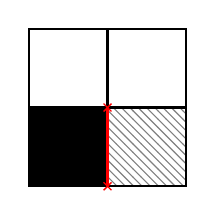
\begin{tikzpicture}
    [
        box/.style={rectangle,draw=black,thick, minimum size=1cm},
    ]
    
    
    here the test 
\foreach \x in {0,1}{
    \foreach \y in {0,1}
        \node[box] at (\x,\y){};
}

\node[box, fill=black] at (0,0){};  
\node[box, pattern = north west lines, pattern color=gray] at (1,0){};  
\draw[step = 1cm, red, thick] (0.5,-0.5) -- (0.5,0.5);
\foreach \x in {0.5}
{
  \draw 
    (\x cm, 0pt) -- (\x cm, 0pt) node[anchor=north] {\scriptsize $\text{\textcolor{red}{}}$};
  \pic[line width=0.5pt,red, rotate = 45] at (\x, 0.5) {mycross};
  \pic[line width=0.5pt,red, rotate = 45] at (\x, -0.5) {mycross};  
}
\end{tikzpicture}
\end{center}
\vspace{-0.25cm}
\caption{The edge $w_{1} = (1,1)$ in red belongs to $C_{2}(0,0) \cap C_{2}(1, 0)$, with the cell $C_{2}(0,0)$ colored in black and $C_{2}(1, 0)$ in gray dashed stripes.}
\label{fig1}
\end{figure}
\vspace{-0.5cm}
Following this consideration, one can define the random quantity
\begin{equation}
f_{t}^{\scriptscriptstyle (i)}(x) := \mathbbm{1}_{\left\{\min\left(X_{x}, X_{\scriptscriptstyle x +e_{i}}\right) < t \leq \max\left(X_{x}, X_{\scriptscriptstyle x+e_{i}}\right)\right\}}
\label{fi}
\end{equation}
to compute the contribution of the edge $w_i(x)$ to the perimeter of the black component of $Z^{\scriptscriptstyle (m)}$.
\begin{Definition}[Perimeter of a binary image $Z^{\scriptscriptstyle (m)}$]\label{defPerimetre}~\\
For $t\in \mathbb{R},$ we denote by $\mathcal{P}_{m}^{\scriptscriptstyle (i)}(t) =~\sum_{x: w_{i}(x) \subset \text{\larger[1]{$($}}0, m \text{\larger[1]{$)$}}^{2}} f_{t}^{\scriptscriptstyle (i)}(x)$ the  sum of all vertical contributions for $i = 1$ and horizontal ones for $i = 2$. Then, the perimeter of the binary image $Z$ is given by
\begin{equation}
\mathcal{P}_{m}(t) := \mathcal{P}_{m}^{\scriptscriptstyle (1)}(t) + \mathcal{P}_{m}^{\scriptscriptstyle (2)}(t).
 \label{eq:6}
\end{equation}
\end{Definition}
% \section{Statistics of the perimeter} 
\section{First moment}
Let us start this study by investigating the first moment of the perimeter.
\begin{Proposition}[First moment of the perimeter] 
\label{propFisrtmoment}
We assume that $\left(X_x \right)_{x \in G_{m}}$ is a stationary Gaussian centered with unit variance random field and $\rho(e_i) = \text{Cov}\left(X_{\scriptscriptstyle 0}, X_{e_i}\right)$ with $\rho(e_i) \in [-1, 1]$. The expected value of the perimeter in \eqref{eq:6} is  given \linebreak by $\mathbb{E}\left(\mathcal{P}_{m}(t)\right) = \mathbb{E}\left(\mathcal{P}^{\scriptscriptstyle  (1)}_{m}(t)\right) + \mathbb{E}\left(\mathcal{P}^{\scriptscriptstyle  (2)}_{m}(t)\right)$  and
if $\rho(e_{i}) \in ]-1,1]$, 
{\small
\begin{align}
\label{propEquationFisrtmoment}
\mathbb{E}\left(f^{(i)}(t) \right) = \mathbb{E}\left(\Phi\left(\dfrac{2t + \sqrt{2(1-\rho(e_i))}|N|}{\sqrt{2(1+\rho(e_i))}}\right)  - \Phi\left(\dfrac{2t - \sqrt{2(1-\rho(e_i))}|N|}{\sqrt{2(1+\rho(e_i))}}\right)\right)
\end{align}}
with $N \sim \mathcal{N}(0,1)$. 
\end{Proposition}
\begin{remark}(degenerative case)
If  $\rho(e_i) = -1, \; \mathbb{E}\left(f^{(i)}(t) \right)= 2\left(1 - \Phi\left(\max\left(0,t\right)\right)\right).$
\end{remark}
\begin{proof}
Let us start with the case where $\rho(e_{i}) \in ]-1,1]$. Considering the formula for $\mathcal{P}^{\scriptscriptstyle  (i)}_{m}(t)$ and applying the stationarity hypothesis, since
\begin{align*}
\left\{ x \in G_{m}; w_{i}(x) \subset (0,m)^{2}\right\} & = \left\{x \in \llbracket 0, m-1 \rrbracket^{2}, (x, x+e_i)\subset (0,m)^{2} \right\} \\ 
& = \left\{ 0, m-1 \right\} \times \left\{ 1, m - 1\right\},
\end{align*}
one can write that, 
\begin{equation}
\mathbb{E}\left(\mathcal{P}^{\scriptscriptstyle  (i)}_{m}(t) \right) = m(m-1)\mathbb{E}\left(f^{(i)}(t)\right).
\label{covarianeproof}
\end{equation}
 with $\mathbb{E}\left(f^{(i)}(t)\right) = \mathbb{P}\left(\min\left(X_{\scriptscriptstyle 0}, X_{e_i}\right) < t \leq \max\left(X_{\scriptscriptstyle 0}, X_{e_i}\right)\right)$. \\
 We start by applying to the Gaussian vector $\left(X_{\scriptscriptstyle 0}, X_{e_i}\right)$ the following transformation \begin{equation} \label{expressions} \Delta^{i}_{\scriptscriptstyle 0} := X_{e_i} - X_{\scriptscriptstyle 0}, \hspace{0.5cm} S^{i}_{\scriptscriptstyle 0} := X_{e_i} + X_{\scriptscriptstyle 0}\end{equation}
The covariance matrix of the new Gaussian vector $\left(\Delta^{\scriptscriptstyle (1)}_{\scriptscriptstyle 0}, S^{\scriptscriptstyle (1)}_{\scriptscriptstyle 0}\right)$ is given by ${\tilde{\Sigma}_{i}(0)~= M\Sigma_{i}(0) M^{\star}}$ with {\small $M = \begin{pmatrix}
-1 & 1 \\
1 & 1  \\
\end{pmatrix}$} and $\Sigma_{i}(0) = \begin{pmatrix} 1 & \rho(e_i) \\
\rho(e_i) & 1  \\ 
\end{pmatrix}.$ \\
Thus, $\tilde{\Sigma}_{i}(0) = \begin{pmatrix}  2(1-\rho(e_i)) & 0 \\ 0 & 2(1+\rho(e_1)  \end{pmatrix}$, which directly  implies that the two variables are independent.
{\small
\begin{align*}
\mathbb{E}\left(f^{(i)}(t)\right) & = \mathbb{P}\left(\min\left(X_{\scriptscriptstyle 0}, X_{e_i}\right) < t \leq \max\left(X_{\scriptscriptstyle 0}, X_{e_i}\right)\right) \\
& = \mathbb{E}\left(\mathbbm{1}_{\left\{\min(X_{\scriptscriptstyle 0}, X_{e_i}) \leq t \leq \max(X_{\scriptscriptstyle 0}, X_{e_i})\right\}}\right) \\
&= \mathbb{E}\left(\mathbbm{1}_{\left\{\min(0, X_{e_i} -X_{\scriptscriptstyle 0}) \leq t -X_{\scriptscriptstyle 0}\leq \max(0, X_{e_i}-X_{0})\right\}}\right) \\
& = \mathbb{E}\left(\mathbbm{1}_{\left\{\min(0, \Delta^{\scriptscriptstyle (i)}_{\scriptscriptstyle 0}) \leq t + \frac{\Delta^{\scriptscriptstyle (i)}_{\scriptscriptstyle 0} - S^{\scriptscriptstyle (i)}_{\scriptscriptstyle 0}}{2}\leq \max(0, \Delta^{\scriptscriptstyle (i)}_{\scriptscriptstyle 0})\right\}}\right) \\
& = \mathbb{E}\left(\mathbbm{1}_{\left\{\min(-\frac{\Delta^{\scriptscriptstyle (i)}_{\scriptscriptstyle 0}}{2}, \frac{\Delta^{\scriptscriptstyle (i)}_{\scriptscriptstyle 0}}{2}) \leq t - \frac{S^{\scriptscriptstyle (i)}_{\scriptscriptstyle 0}}{2}\leq \max(-\frac{\Delta^{\scriptscriptstyle (i)}_{\scriptscriptstyle 0}}{2}, \frac{\Delta^{\scriptscriptstyle (i)}_{\scriptscriptstyle 0}}{2})\right\}}\right) \\
& = \mathbb{E}\left(\mathbbm{1}_{\left\{ \left|2t - S^{\scriptscriptstyle (1)}_{\scriptscriptstyle 0}\right| \leq \left|\Delta^{\scriptscriptstyle (1)}_{\scriptscriptstyle 0}\right|\right\}}\right). \\
& = \mathbb{E}\left(\mathbbm{1}_{\left\{\frac{2t - \sqrt{2(1-\rho(e_i))}|N|}{\sqrt{2(1+\rho(e_i))}}  \leq Y \leq \frac{2t + \sqrt{2(1-\rho(e_i))}|N|}{\sqrt{2(1+\rho(e_i))}}\right\}}\right)
\end{align*}}  
with $N, Y \sim \mathcal{N}(0,I_{2})$, thus 
$$\mathbb{E}\left(f^{(i)}(t)\right) = \mathbb{E}\left(\Phi\left(\dfrac{2t + \sqrt{2(1-\rho(e_i))}|N|}{\sqrt{2(1+\rho(e_i))}}\right)  - \Phi\left(\dfrac{2t - \sqrt{2(1-\rho(e_i))}|N|}{\sqrt{2(1+\rho(e_i))}}\right)\right).$$
Let us now consider the case where $\rho(e_i) = -1$. Then there exists $N \sim \mathcal{N}\left(0,1\right)$ such that $\left(X_{\scriptscriptstyle 0}, X_{e_i}\right) \overset{d}{=} \left(N, -N\right)$. Thus, 
\begin{align*}
\mathbb{P}\left(\min\left(X_{\scriptscriptstyle 0}, X_{e_i}\right) < t \leq \max\left(X_{\scriptscriptstyle 0}, X_{e_i}\right)\right) & = \mathbb{P}\left(\min\left(N, -N\right) < t \leq \max\left(N, -N\right)\right) \\
& \hspace{-6cm}= \mathbb{P}\left(-|N| < t \leq |N|\right) = \cfrac{2}{\sqrt{2\pi}} \int_{\scriptscriptstyle 0}^{+\infty} \mathbbm{1}_{\left\{-z < t \leq z\right\}} e^{-\frac{z^2}{2}}dz  = \cfrac{2}{\sqrt{2\pi}} \int_{\scriptscriptstyle 0}^{+\infty} \mathbbm{1}_{\left\{t \leq z\right\}} e^{-\frac{z^2}{2}}dz \\
& \hspace{-6cm}= 2\left(1 - \Phi\left(\max\left(0,t\right)\right)\right).
\end{align*}
\end{proof}
Note that this result extends those given in \cite{HermineAgnes} (Proposition 3) since we do not assume here that $\rho(e_i) > 0$. 

\begin{remark}
\label{iidCase}
In the independent case, $\rho(e_i) = 0$, we can write
{\small
\begin{align*}
\mathbb{E}\left(\mathcal{P}^{\scriptscriptstyle  (i)}_{m}(t) \right) & = m(m-1)\mathbb{E}\left(\Phi\left(\sqrt{2}t + |Z|\right) - \Phi\left(\sqrt{2}t - |Z|\right)\right) = 2m(m-1)\Phi(t)\left(1-\Phi(t)\right) 
\end{align*}}
by applying a variable change {\small$\left\{\begin{array}{rcl}
u & = & \frac{y - z}{\sqrt{2}} \\
v & = & \frac{y+z}{\sqrt{2}} \\
\end{array}\right.$}, we get the same result as in \cite{Psymetrie} (Proposition \textcolor{blue}{3.1}).
\end{remark}
\begin{remark}
In order to have convergence when $m \to \infty$, one has to consider the normalise perimeter with the area of the window ($m^2$).
\end{remark}
The total variation of an image $u \in L^{1}_{loc}(\Omega)$ is given by $\int_{\Omega}|\nabla u|dx$ which is equal by the coarea formula to $\int_{\mathbb{R}}\mathcal{P}(t)dt$.
\begin{Proposition}
Under the assumptions stated in Proposition \ref{propFisrtmoment}, we get 
\begin{equation}
\label{totalvariation}
\int_{\mathbb{R}} \mathbb{E}\left(\mathcal{P}^{(i)}_{m}(t)\right) dt = \frac{2m(m-1)}{\sqrt{\pi}}\left(\sqrt{1-\rho(e_i)}  \right).
\end{equation}
\end{Proposition}
\begin{proof}
Using the result stated in Proposition \ref{propFisrtmoment}, we get that $\mathbb{E}\left(\mathcal{P}^{\scriptscriptstyle  (i)}_{m}(t) \right)$ is equal to,
{\small
\begin{align*}
\int_{\mathbb{R}} \mathbb{E}\left(\mathcal{P}^{(i)}_{m}(t)\right) dt & = \\
& \hspace{-2cm}\cfrac{m(m-1)}{\sqrt{2\pi}} \int_{\mathbb{R}}\int_{\mathbb{R}} \left(\Phi\left(\dfrac{\sqrt{2}t + \sqrt{1-\rho(e_i)}|u|}{\sqrt{1+\rho(e_i)}}\right) - \Phi\left(\dfrac{\sqrt{2}t - \sqrt{1-\rho(e_i)}|u|}{\sqrt{1+\rho(e_i)}}\right)\right)e^{-\frac{1}{2}u^2}dudt \\
& \hspace{-2cm}=\cfrac{m(m-1)}{2\pi} \int_{\mathbb{R}}\int_{\mathbb{R}}\int_{\mathbb{R}} e^{-\frac{1}{2}u^2}e^{-\frac{1}{2}v^2} \mathbbm{1}_{\left\{\dfrac{\sqrt{2}t - \sqrt{1-\rho(e_i)}|u|}{\sqrt{1+\rho(e_i)}}\leq v \leq\dfrac{\sqrt{2}t + \sqrt{1-\rho(e_i)}|u|}{\sqrt{1+\rho(e_i)}}\right\}} du dv dt ,\\
& \hspace{-2cm}\text{using Fubini-Tonelli Theorem,} \\
& \hspace{-2cm}= \cfrac{m(m-1)}{2\pi}\int_{\mathbb{R}}\int_{\mathbb{R}} e^{-\frac{1}{2}u^2}e^{-\frac{1}{2}v^2} \\
& \hspace{-2cm} \left(\int_{\mathbb{R}} \mathbbm{1}_{\left\{\dfrac{\sqrt{1+\rho(e_i)}v - \sqrt{1-\rho(e_i)}|u|}{\sqrt{2}}\leq t\leq\dfrac{\sqrt{1+\rho(e_i)}v + \sqrt{1-\rho(e_i)}|u|}{\sqrt{2}}\right\}} dt\right) du dv \\
& \hspace{-2cm}= \cfrac{m(m-1)}{2\pi} \int_{\mathbb{R}}\int_{\mathbb{R}} e^{-\frac{1}{2}u^2}e^{-\frac{1}{2}v^2}\left(\dfrac{2|u|\sqrt{1-\rho(e_i)}}{\sqrt{2}}\right)dudv = \frac{2\sqrt{1-\rho(e_i)}}{\sqrt{2}} m(m-1)\underbrace{\mathbb{E}(|U|)}_{\sqrt{\frac{2}{\pi}}}\\
&\hspace{-2cm}=\frac{2}{\sqrt{\pi}}m(m-1)\sqrt{1-\rho(e_i)}.
\end{align*}
}
\end{proof}
\begin{remark}
The first moment of the total variation is given by the sum over the two directions of Equation \eqref{totalvariation}. 
\end{remark}
\begin{remark}
Using this result, one can define an estimator for $\rho(e_i)$. 
\end{remark}
Study of the behavior of the nodal curve $t = 0$, 
\begin{remark}
\label{decreasingrho}
Considering $\tilde{\rho}(e_i), \bar{\rho}(e_i)$ two covariance, we  have the following result 
\begin{equation*}
 \text{if} \hspace{0.5cm} \tilde{\rho}(e_i) < \bar{\rho}(e_i) \hspace{0.5cm} \text{then} \hspace{0.5cm}\mathbb{E}\left(\mathcal{P}^{\scriptscriptstyle (i)}_{m, \tilde{\rho}}(0)\right) > \mathbb{E}\left(\mathcal{P}^{\scriptscriptstyle (i)}_{m, \bar{\rho}}(0)\right).
\end{equation*}
Where $\mathcal{P}^{\scriptscriptstyle (i)}_{m, \tilde{\rho}}$ is the perimeter with respect of the orientation $i$ associated to the Gaussian field of covariance $\tilde{\rho}$. 
\end{remark}
\begin{proof}
Note that $\rho \mapsto \sqrt{1-\rho}$ is strictly decreasing similarly  for level $0$, one has $\mathbb{E}\left(f^{(i)}(0)\right) = \mathbb{E}\left(\frac{\sqrt{1-\rho(e_i)}}{\sqrt{1+\rho(e_i)}}|N|\right) - \mathbb{E}\left(-\frac{\sqrt{1-\rho(e_i)}}{\sqrt{1+\rho(e_i)}}|N|\right) = 2\mathbb{E}\left(\frac{\sqrt{1-\rho(e_i)}}{\sqrt{1+\rho(e_i)}}|N|\right) - 1$, since $\rho \mapsto \frac{\sqrt{1-\rho}}{\sqrt{1+\rho}}$ is strictly decreasing, we see that $\rho \mapsto 2\mathbb{E}\left(\frac{\sqrt{1-\rho}}{\sqrt{1+\rho}}|N|\right) - 1 $ is also strictly decreasing. 
\end{proof}
\textcolor{blue}{reorient toward Github for illustrations.}
\section{Covariance of the perimeter for two thresholds}
Let $s, t \in \mathbb{R}$ such that $t \leq s$. Let us consider a stationary Gaussian random field $\left(X_{\scriptscriptstyle x}\right)_{x \in G_{m}}$ with zero mean and unit variance whose covariance structure is given by $\rho(x) = \text{Cov}\left(X_{\scriptscriptstyle 0}, X_{\scriptscriptstyle x}\right)$.
\begin{Lemma} 
\label{CovLemma}
\begin{align}
\text{Cov}(\mathcal{P}_{m}(t), \mathcal{P}_{m}(s))  & = \text{Cov}(\mathcal{P}_{m}^{\scriptscriptstyle (1)}(t), \mathcal{P}_{m}^{\scriptscriptstyle (1)}(s)) + 2\text{Cov}(\mathcal{P}_{m}^{\scriptscriptstyle (1)}(t), \mathcal{P}_{m}^{\scriptscriptstyle (2)}(s)) + \text{Cov}(\mathcal{P}_{m}^{\scriptscriptstyle (2)}(t), \mathcal{P}_{m}^{\scriptscriptstyle (2)}(s)) .
\label{covariance}
\end{align} 
With 
\begin{align*}
\text{Cov}\left(\mathcal{P}_{m}^{\scriptscriptstyle (i)}(t),\mathcal{P}_{m}^{\scriptscriptstyle (i)}(s) \right) 
& = \sum_{x_{\scriptscriptstyle 1}=\left(1-m\right)}^{m-1}\sum_{x_{\scriptscriptstyle 2}=\left(2-m\right)}^{m-2}\left(m -|x_{1}|\right)\left(m - 1- |x_{2}|\right) \text{Cov}\left(f_{t}^{\scriptscriptstyle (i)}(0), f_{s}^{\scriptscriptstyle (i)}(x) \right) 
\end{align*} 
and 
\begin{align*}
\text{Cov}\left(\mathcal{P}_{m}^{\scriptscriptstyle (1)}(t),\mathcal{P}_{m}^{\scriptscriptstyle (2)}(s) \right) & = \sum_{x_1 = 0}^{m-2} \sum_{x_2=1}^{m-1}\left(m-x_1-1\right)\left(m-x_2\right)\text{Cov}\left(f_{t}^{\scriptscriptstyle (1)}(0), f_{s}^{ \scriptscriptstyle (2)}(x) \right)\\
& + \sum_{x_1 = 0}^{m-2} \sum_{x_2=2-m}^{\scriptscriptstyle 0}\left(m-x_1-1\right)\left(m+x_2-1\right)\text{Cov}\left(f_{t}^{\scriptscriptstyle (1)}(0), f_{s}^{ \scriptscriptstyle (2)}(x) \right)\\
& + \sum_{x_1 = -m+1}^{-1} \sum_{x_2=1}^{m-1}\left(m+x_1\right)\left(m-x_2\right)\text{Cov}\left(f_{t}^{\scriptscriptstyle (1)}(0), f_{s}^{ \scriptscriptstyle (2)}(x) \right)\\
& + \sum_{x_1 = -m+1}^{-1} \sum_{x_2=2-m}^{\scriptscriptstyle 0}\left(m+x_1\right)\left(m+x_2-1\right)\text{Cov}\left(f_{t}^{\scriptscriptstyle (1)}(0), f_{s}^{ \scriptscriptstyle (2)}(x) \right) 
\end{align*}
\end{Lemma}
\begin{proof}
To simplify the notations, we chose to do the computations for direction $i =1$. Let us start with the computation of $\text{Cov}(\mathcal{P}_{m}^{\scriptscriptstyle (1)}(t), \mathcal{P}_{m}^{\scriptscriptstyle (1)}(s))$ for $t \leq s$. 
\begin{align*}
\text{Cov}(\mathcal{P}_{m}^{\scriptscriptstyle (1)}(t), \mathcal{P}_{m}^{\scriptscriptstyle (1)}(s))& = \text{Cov}\left( \sum_{x, w_{1}(x) \subset \text{\larger[1]{$($}}0, m \text{\larger[1]{$)$}}^{2}}f_{t}^{\scriptscriptstyle (1)}(x), \sum_{y, w_{1}(y) \subset \text{\larger[1]{$($}}0, m \text{\larger[1]{$)$}}^{2}} f_{s}^{\scriptscriptstyle (1)}(y)\right) \\
& = \sum_{x, w_{1}(x) \subset \text{\larger[1]{$($}}0, m \text{\larger[1]{$)$}}^{2}} \sum_{y, w_{1}(y) \subset \text{\larger[1]{$($}}0, m \text{\larger[1]{$)$}}^{2}} \text{Cov}\left(f_{t}^{\scriptscriptstyle (1)}(x), f_{s}^{\scriptscriptstyle (1)}(y) \right).
\end{align*}
By the stationarity hypothesis, one has $\text{Cov}\left(f_{t}^{\scriptscriptstyle (1)}(x), f_{s}^{\scriptscriptstyle (1)}(y) \right)= \text{Cov}\left(f_{t}^{\scriptscriptstyle (1)}(0), f_{s}^{\scriptscriptstyle (1)}(y-x) \right)$. Then 
\begin{align*}
\text{Cov}\left(\mathcal{P}_{m}^{\scriptscriptstyle (1)}(t),\mathcal{P}_{m}^{\scriptscriptstyle (1)}(s) \right) & = \sum_{x_1 = 0}^{m-1}\sum_{x_2 = 1}^{m-1}\sum_{y_1 = 0}^{m-1}\sum_{y_2 = 1}^{m-1} \text{Cov}\left(f_{t}^{\scriptscriptstyle (1)}(0), f_{s}^{ \scriptscriptstyle (1)}(y-x) \right)
\end{align*}
for $x_1 \in [0,m-1]$ and $z_1 = y_1 - x_1$ one has
\begin{align*} 
\left\{
\begin{array}{rcl}
0 \leq x_1 \leq m-1 \\
0 \leq y_1 \leq m-1 
\end{array}\right.& \implies  \left\{ \begin{array}{rcl}
0 \leq x_1 \leq m-1 \hspace{0.7cm} \\
-x_1 \leq z_1 \leq m-1 - x_1
\end{array}\right. \\
& \implies  \left\{
\begin{array}{rcl}
1-m \leq z_1 \leq m-1 \hspace{2.5cm}  \\
\max(0, -z_1) \leq x_1 \leq \min(m-1 , m-1-z_1)
\end{array}\right..
\end{align*} 
Similarly for $z_2 = y_2 - x_2$ and $x_2 \in [1, m-1]$
\begin{align*}
 \left\{
\begin{array}{rcl}
1 \leq x_2 \leq m-1 \\
1 \leq y_2 \leq m-1 
\end{array}\right. & \implies
\left\{
\begin{array}{rcl}
2-m \leq z_2 \leq m-2 \hspace{2.5cm}  \\
\max(1, 1-z_2) \leq x_2 \leq \min(m-1 , m-1-z_2).
\end{array}\right., 
\end{align*}
Thus,
\begin{align*}
\text{Cov}\left(\mathcal{P}_{m}^{\scriptscriptstyle (1)}(t),\mathcal{P}_{m}^{\scriptscriptstyle (1)}(s) \right) &  = \sum_{z_{\scriptscriptstyle 1} = \left(1-m\right)}^{m-1}\sum_{z_{\scriptscriptstyle 2}=\left(2-m\right)}^{m-2}\left(m -|z_{1}|\right)\left(m - 1- |z_{2}|\right) \text{Cov}\left(f_{t}^{\scriptscriptstyle (1)}(0), f_{s}^{\scriptscriptstyle (1)}(z) \right) 
\end{align*}
For the second part of \eqref{covariance}, we have still by stationarity
\begin{align*}
\text{Cov}\left(\mathcal{P}_{m}^{\scriptscriptstyle (1)}(t),\mathcal{P}_{m}^{\scriptscriptstyle (2)}(s) \right) & = \sum_{x, w_{1}(x) \subset \text{\larger[1]{$($}}0, m \text{\larger[1]{$)$}}^{2}} \sum_{y, w_{2}(y) \subset \text{\larger[1]{$($}}0, m \text{\larger[1]{$)$}}^{2}} \text{Cov}\left(f_{t}^{\scriptscriptstyle (1)}(0), f_{s}^{ \scriptscriptstyle (2)}(y-x) \right)\\
& =  \sum_{x_1 = 0}^{m-1}\sum_{x_2 = 1}^{m-1}\sum_{y_1 = 1}^{m-1}\sum_{y_2 = 0}^{m-1}\text{Cov}\left(f_{t}^{\scriptscriptstyle (1)}(0), f_{s}^{ \scriptscriptstyle (2)}(y-x) \right)
\end{align*}
Again, considering $z_1 = y_1 - x_1$
\begin{align*} 
\left\{
\begin{array}{rcl}
0 \leq x_1 \leq m-1 \\
1 \leq y_1 \leq m-1 
\end{array}\right.& \implies  \left\{ \begin{array}{rcl}
0 \leq x_1 \leq m-1 \hspace{0.7cm} \\
1 -x_1 \leq z_1 \leq m- 1 - x_1
\end{array}\right. \\
& \implies  \left\{
\begin{array}{rcl}
2 - m \leq z_1 \leq m-1 \hspace{2.5cm}  \\
\max(0, 1-z_1) \leq x_1 \leq \min(m-1 , m-1-z_1),
\end{array}\right.
\end{align*} 
and, $z_{2} = y_{2}-x_{2}$
\begin{align*} 
\left\{
\begin{array}{rcl}
1 \leq x_2 \leq m-1 \\
0 \leq y_2 \leq m-1 
\end{array}\right.& \implies  \left\{ \begin{array}{rcl}
1 \leq x_2 \leq m-1 \hspace{0.7cm} \\
-x_2 \leq z_2 \leq m- 1 - x_2
\end{array}\right. \\
& \implies  \left\{
\begin{array}{rcl}
1 - m \leq z_2 \leq m-2 \hspace{2.5cm}  \\
\max(1, -z_2) \leq x_2 \leq \min(m-1 , m-1-z_2)
\end{array}\right..
\end{align*} 
Thus, 
\begin{align*}
\text{Cov}\left(\mathcal{P}_{m}^{\scriptscriptstyle (1)}(t),\mathcal{P}_{m}^{\scriptscriptstyle (2)}(s) \right) & = \sum_{z_2 = 0}^{m-2} \sum_{z_1=1}^{m-1}\left(m-z_2-1\right)\left(m-z_1\right)\text{Cov}\left(f_{t}^{\scriptscriptstyle (1)}(0), f_{s}^{ \scriptscriptstyle (2)}(z) \right)\\
& + \sum_{z_2 = 0}^{m-2} \sum_{z_1=2-m}^{\scriptscriptstyle 0}\left(m-z_2-1\right)\left(m+z_1-1\right)\text{Cov}\left(f_{t}^{\scriptscriptstyle (1)}(0), f_{s}^{ \scriptscriptstyle (2)}(z) \right)\\
& + \sum_{z_2 = -m+1}^{-1} \sum_{z_1=1}^{m-1}\left(m+z_2\right)\left(m-z_1\right)\text{Cov}\left(f_{t}^{\scriptscriptstyle (1)}(0), f_{s}^{ \scriptscriptstyle (2)}(z) \right)\\
& + \sum_{z_2 = -m+1}^{-1} \sum_{z_1=2-m}^{\scriptscriptstyle 0}\left(m+z_2\right)\left(m+z_1-1\right)\text{Cov}\left(f_{t}^{\scriptscriptstyle (1)}(0), f_{s}^{ \scriptscriptstyle (2)}(z) \right) 
\end{align*}
\end{proof}
Getting the value of the covariance requires the computation of all the elements of the sum, let us first start with the term $\text{Cov}\left(f_{t}^{\scriptscriptstyle (1)}(0), f_{s}^{\scriptscriptstyle (1)}(0)\right)$,
\begin{Lemma}
The case $x=0$ is a special case, in order to compute it, we just have to apply the same strategy we used to compute the first moment in \ref{propFisrtmoment}, thus we get,
\begin{align*}
\text{Cov}\left(f_{t}^{\scriptscriptstyle (1)}(0), f_{s}^{\scriptscriptstyle (1)}(0)\right) & = \mathbb{E}\left(\mathbbm{1}_{\left\{\min(X_{\scriptscriptstyle 0}, X_{\scriptscriptstyle  e_1}) \leq t \leq \max(X_{\scriptscriptstyle 0}, X_{e_1})\right\}}\mathbbm{1}_{\left\{\min(X_{\scriptscriptstyle 0}, X_{ \scriptscriptstyle  e_1}) \leq s \leq \max(X_{\scriptscriptstyle 0}, X_{\scriptscriptstyle e_1}) \right\}}\right) \\
& - \mathbb{E}\left(\mathbbm{1}_{\left\{\min(X_{\scriptscriptstyle 0}, X_{e_1}) \leq t \leq \max(X_{\scriptscriptstyle 0}, X_{e_1})\right\}}\right)\mathbb{E}\left(\mathbbm{1}_{\left\{\min(X_{\scriptscriptstyle 0}, X_{e_1}) \leq s \leq \max(X_{\scriptscriptstyle 0}, X_{e_1})\right\}}\right).
\end{align*}
And, 
{\small
\begin{align*}
\mathbb{E}\left(\mathbbm{1}_{\left\{\min(X_{\scriptscriptstyle 0}, X_{\scriptscriptstyle  e_1}) \leq t \leq \max(X_{\scriptscriptstyle 0}, X_{e_1})\right\}}\mathbbm{1}_{\left\{\min(X_{\scriptscriptstyle 0}, X_{ \scriptscriptstyle  e_1}) \leq s \leq \max(X_{\scriptscriptstyle 0}, X_{\scriptscriptstyle e_1}) \right\}}\right) & = \\
& \hspace{-9cm}\mathbb{E}\left(\left(\Phi\left(\dfrac{\sqrt{2}\max\left(t,s\right) + \sqrt{1-\rho(e_1)}|Z|}{\sqrt{1+\rho(e_1)}}\right)  - \Phi\left(\dfrac{\sqrt{2}\min\left(t,s\right) - \sqrt{1-\rho(e_1)}|Z|}{\sqrt{1+\rho(e_1)}}\right)\right)\right. \\
& \hspace{-1cm} \left.\mathbbm{1}_{\left\{(|s-t| \leq |Z|\sqrt{2(1-\rho(e_1))}\right\}}\right)
\end{align*}}
with $Z \sim \mathcal{N}(0,1)$. 
\end{Lemma}
\subsection{Three and four cells configuration}
Figure \ref{configurations} shows the four types of configurations that are encountered in the computation of $\text{Cov}\left(f_{t}^{\scriptscriptstyle (1)}(0), f_{s}^{ \scriptscriptstyle (i)}(x)\right)$ in Lemma \ref{CovLemma} depending on the orientation $i$ and position on the grid $x$. We will call \textit{three cells} and \textit{four cells} configuration depending on how many cells are involved. 
\begin{figure}[H]
\begin{center}
  \captionsetup[subfigure]{justification=centering}
  \begin{subfigure}[b]{0.25\textwidth} 
  \centering
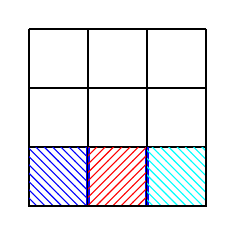
\begin{tikzpicture}[scale = 1.5]
\draw[step = 0.5cm, black, thick](0,0) grid (1.5,1.5);
\draw[step = 2cm, line width =0.5mm, blue] (0.5,0) -- (0.5,0.5);
\draw[step = 2cm, line width =0.5mm, blue] (1,0) -- (1,0.5);
\draw[pattern=north west lines, pattern color=blue] (0,0) rectangle (0.5,0.5);
\draw[pattern=north east lines, pattern color=red] (0.5, 0) rectangle (1,0.5);
\draw[pattern=north west lines, pattern color=cyan, opacity=1] (1, 0) rectangle (1.5,0.5);
\end{tikzpicture}
\caption{$i = 1$, $x = (0,1)$}
\end{subfigure}
  \hspace{0.5cm}
  \begin{subfigure}[b]{0.25\textwidth} 
  \centering
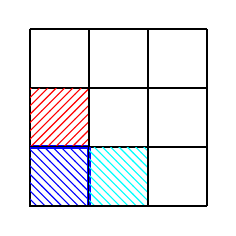
\begin{tikzpicture}[scale =1.5]
\draw[step = 0.5cm, black, thick](0,0) grid (1.5,1.5);
\draw[step = 2cm, line width =0.5mm, blue] (0.5,0) -- (0.5,0.5);
\draw[step = 2cm, line width =0.5mm, blue] (0,0.5) -- (0.5,0.5);
\draw[pattern=north west lines, pattern color=blue] (0,0) rectangle (0.5,0.5);
\draw[pattern=north east lines, pattern color=red] (0, 0.5) rectangle (0.5,1);
\draw[pattern=north west lines, pattern color=cyan, opacity=1] (0.5, 0) rectangle (1,0.5);
\end{tikzpicture}
\caption{$i = 2, x = (0,0)$}
\end{subfigure}
~\\
\begin{subfigure}[b]{0.25\textwidth} 
\centering 
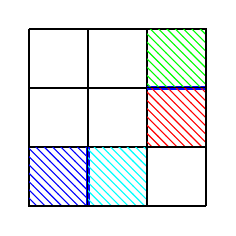
\begin{tikzpicture}[scale = 1.5]
\draw[step = 0.5cm, black, thick](0,0) grid (1.5,1.5);
\draw[step = 2cm, line width =0.5mm, blue] (0.5,0) -- (0.5,0.5);
\draw[step = 2cm, line width =0.5mm, blue] (1,1) -- (1.5,1);
\draw[pattern=north west lines, pattern color=blue] (0,0) rectangle (0.5,0.5);
\draw[pattern=north west lines, pattern color=cyan, opacity=1] (0.5, 0) rectangle (1,0.5);
\draw[pattern=north west lines, pattern color=green, opacity=1] (1.5, 1.5) rectangle (1,1);
\draw[pattern=north west lines, pattern color=red, opacity=1] (1, 0.5)  rectangle (1.5, 1);
\end{tikzpicture}
\caption{$i = 2, z = (2,1)$}
\end{subfigure}
  \hspace{0.5cm}
  \begin{subfigure}[b]{0.25\textwidth} 
  \centering 
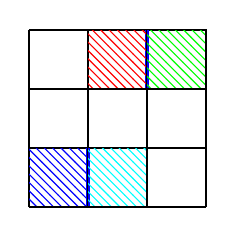
\begin{tikzpicture}[scale = 1.5]
\draw[step = 0.5cm, black, thick](0,0) grid (1.5,1.5);
\draw[step = 2cm, line width =0.5mm, blue] (0.5,0) -- (0.5,0.5);
\draw[step = 2cm, line width =0.5mm, blue] (1,1) -- (1,1.5);
\draw[pattern=north west lines, pattern color=blue] (0,0) rectangle (0.5,0.5);
\draw[pattern=north west lines, pattern color=cyan, opacity=1] (0.5, 0) rectangle (1,0.5);
\draw[pattern=north west lines, pattern color=green, opacity=1] (1.5, 1.5) rectangle (1,1);
\draw[pattern=north west lines, pattern color=red, opacity=1] (0.5, 1)  rectangle (1, 1.5);
\end{tikzpicture}
\caption{$i = 1, x = (1,2)$}
\end{subfigure}
\end{center}
\caption{Illustration of the three cells and four cells configuration (respectively first and second row) involved in the study of $\text{Cov}\left(f_{t}^{\scriptscriptstyle (1)}(0), f_{s}^{ \scriptscriptstyle (i)}(x)\right)$ in Lemma \ref{CovLemma}.}
\label{configurations}
\end{figure}
Let us consider the Gaussian vector $\left(X_{\scriptscriptstyle 0}, X_{e_1}, X_{\scriptscriptstyle x}, X_{x+e_i}\right)$ of covariance matrix given by $$\Sigma_{i}(x) = \begin{pmatrix} 1 & \rho(e_1) & \rho(x) & \rho(x+e_i)\\
\rho(e_1) & 1 & \rho(x-e_1) &  \rho(x+e_i- e_1) \\ 
\rho(x) & \rho(x-e_1) & 1 & \rho(e_i) \\
\rho(x+e_i) & \rho(x+e_i-e_1) & \rho(e_i) & 1 \end{pmatrix}.$$ 
Let us define the following quantity  \begin{equation} \label{expressions} \Delta^{i}_{\scriptscriptstyle x} := X_{x+e_i} - X_{\scriptscriptstyle x}, \hspace{0.5cm} S^{i}_{\scriptscriptstyle x} := X_{x+e_i} + X_{\scriptscriptstyle x}\end{equation} and 
{\small
$\left\{\begin{array}{rlc}
\Delta \rho(x) & = & \rho(x-e_1)-\rho(x) \\
S\rho(x) & = & \rho(x-e_1)+\rho(x)\\
\Delta \rho(x+e_i) & = & \rho(x+e_i-e_1)-\rho(x+e_i) \\
S\rho(x+e_i) & = & \rho(x+e_i-e_1)+\rho(x+e_i)\\
\end{array}\right.\\
$
}
The covariance matrix of the Gaussian vector $\left(\Delta^{\scriptscriptstyle (1)}_{\scriptscriptstyle 0}, S^{\scriptscriptstyle (1)}_{\scriptscriptstyle 0}, \Delta^{\scriptscriptstyle (i)}_{\scriptscriptstyle x}, S^{\scriptscriptstyle (i)}_{\scriptscriptstyle x}\right)$ is equal to ${\tilde{\Sigma}~= M\Sigma M^{\star}}$ with {\small $M = \begin{pmatrix}
-1 & 1 & 0 &  0 \\
1 & 1 & 0 &  0 \\
0& 0 & -1 &  1 \\
0 & 0 & 1 & 1
\end{pmatrix}$}. \\
Then $\tilde{\Sigma} = \begin{pmatrix} A_{1} & B \\ B^{\star} & A_{i} \end{pmatrix}$
with 
$A_{i} = \begin{pmatrix} 2(1-\rho(e_i)) & 0 \\ 0 & 2(1+\rho(e_i))\end{pmatrix}$ \\
and {\small $B = \begin{pmatrix} \Delta \rho(x+e_i) - \Delta \rho(x)&    \Delta \rho(x) + \Delta \rho(x+e_i) \\ 
 S\rho(x+e_i)- S\rho(x) &  S\rho(x) + S\rho(x+e_i) 
 \end{pmatrix}$}. \\
The quantity we aim to compute is 
{\small
\begin{align}
\label{covconf}
\text{Cov}\left(f_{t}^{\scriptscriptstyle (1)}(0), f_{s}^{ \scriptscriptstyle (i)}(x)\right) & = \nonumber \\
& \hspace{-2.7cm} \mathbb{E}\left(\mathbbm{1}_{\left\{\min(X_{\scriptscriptstyle 0}, X_{e_1}) \leq t \leq \max(X_{\scriptscriptstyle 0}, X_{e_1})\right\}}\mathbbm{1}_{\left\{\min(X_{\scriptscriptstyle x}, X_{x+e_i}) \leq s \leq \max(X_{\scriptscriptstyle x}, X_{x+e_i}) \right\}}\right) \nonumber\\
& \hspace{1cm} - \mathbb{E}\left(\mathbbm{1}_{\left\{\min(X_{\scriptscriptstyle 0}, X_{e_1}) \leq t \leq \max(X_{\scriptscriptstyle 0}, X_{e_1})\right\}}\right)\mathbb{E}\left(\mathbbm{1}_{\left\{\min(X_{\scriptscriptstyle 0}, X_{e_i}) \leq t \leq \max(X_{\scriptscriptstyle 0}, X_{e_i})\right\}}\right).
\end{align}}Considering the first part of the previous equation, 
{\small
\begin{align*}
\mathbb{E}\left(\mathbbm{1}_{\left\{\min(X_{\scriptscriptstyle 0}, X_{e_1}) \leq t \leq \max(X_{\scriptscriptstyle 0}, X_{e_1})\right\}}\mathbbm{1}_{\left\{\min(X_{\scriptscriptstyle x}, X_{x+e_i}) \leq s \leq \max(X_{\scriptscriptstyle x}, X_{x+e_i}) \right\}}\right) \\
& \hspace{-9.75cm}= \mathbb{E}\left(\mathbbm{1}_{\left\{\min(0, X_{e_1} -X_{\scriptscriptstyle 0}) \leq t -X_{\scriptscriptstyle 0}\leq \max(0, X_{e_1}-X_{\scriptscriptstyle 0})\right\}}\mathbbm{1}_{\left\{\min(0, X_{x+e_i}-X_{\scriptscriptstyle x}) \leq s - X_{\scriptscriptstyle x} \leq \max(0, X_{x+e_i} - X_{\scriptscriptstyle x}) \right\}}\right) \\
& \hspace{-9.75cm}= \mathbb{E}\left(\mathbbm{1}_{\left\{\min(0, \Delta^{\scriptscriptstyle (1)}_{\scriptscriptstyle 0}) \leq t + \frac{\Delta^{\scriptscriptstyle (1)}_{\scriptscriptstyle 0} - S^{\scriptscriptstyle (1)}_{\scriptscriptstyle 0}}{2}\leq \max(0, \Delta^{\scriptscriptstyle (1)}_{\scriptscriptstyle 0})\right\}}\mathbbm{1}_{\left\{\min(0, \Delta^{\scriptscriptstyle (i)}_{\scriptscriptstyle x}) \leq s + \frac{\Delta^{\scriptscriptstyle (i)}_{\scriptscriptstyle x} - S^{i}_{\scriptscriptstyle x}}{2} \leq \max(0, \Delta^{\scriptscriptstyle (i)}_{\scriptscriptstyle x}) \right\}}\right) \\
& \hspace{-9.75cm}= \mathbb{E}\left(\mathbbm{1}_{\left\{\min(-\frac{\Delta^{\scriptscriptstyle (1)}_{\scriptscriptstyle 0}}{2}, \frac{\Delta^{\scriptscriptstyle (1)}_{\scriptscriptstyle 0}}{2}) \leq t - \frac{S^{\scriptscriptstyle (1)}_{\scriptscriptstyle 0}}{2}\leq \max(-\frac{\Delta^{\scriptscriptstyle (1)}_{\scriptscriptstyle 0}}{2}, \frac{\Delta^{\scriptscriptstyle (1)}_{\scriptscriptstyle 0}}{2})\right\}}\mathbbm{1}_{\left\{\min(-\frac{\Delta^{\scriptscriptstyle (i)}_{\scriptscriptstyle x}}{2}, \frac{\Delta^{\scriptscriptstyle (i)}_{\scriptscriptstyle x}}{2}) \leq s - \frac{S^{i}_{\scriptscriptstyle x}}{2} \leq \max(-\frac{\Delta^{\scriptscriptstyle (i)}_{\scriptscriptstyle x}}{2},\frac{\Delta^{\scriptscriptstyle (i)}_{\scriptscriptstyle x}}{2}) \right\}}\right) \\
& \hspace{-9.75cm}= \mathbb{E}\left(\mathbbm{1}_{\left\{ \left|2t - S^{\scriptscriptstyle (1)}_{\scriptscriptstyle 0}\right| \leq \left|\Delta^{\scriptscriptstyle (1)}_{\scriptscriptstyle 0}\right|\right\}}\mathbbm{1}_{\left\{ \left|2s - S^{\scriptscriptstyle (i)}_{\scriptscriptstyle x}\right| \leq \left|\Delta^{\scriptscriptstyle (i)}_x\right| \right\}}\right).
\end{align*}}Let us assume that $|\rho(e_1)| < 1$, the Cholesky decomposition of $\Sigma_{i}(x)$ allows us to get the expression of the Gaussian vector $\left(\Delta^{\scriptscriptstyle (1)}_{\scriptscriptstyle 0},S^{\scriptscriptstyle (1)}_{\scriptscriptstyle 0},\Delta^{\scriptscriptstyle (i)}_{\scriptscriptstyle x},S^{\scriptscriptstyle (i)}_{\scriptscriptstyle x} \right)$ in a new basis $\left(U,V,W,Z\right)$ with $\left(U, V, W, Z\right) \sim \mathcal{N}\left(0,I_{4}\right)$. We get the following decomposition \\ 
$\left\{
  \begin{array}{rlc}
  \Delta^{\scriptscriptstyle (1)}_{\scriptscriptstyle 0} & = & \sigma_1U, \\
  S^{\scriptscriptstyle (1)}_{\scriptscriptstyle 0} & = & \sigma_2V, \\
  \Delta^{\scriptscriptstyle (i)}_{\scriptscriptstyle  x}& = &  \alpha^{\scriptscriptstyle(i)}_{U}(x)U +  \alpha^{\scriptscriptstyle(i)}_{V}(x) V +  \alpha^{\scriptscriptstyle(i)}_{W}(x) W, \\
  S^{\scriptscriptstyle (i)}_{\scriptscriptstyle x} & = &    \pi^{\scriptscriptstyle(i)}_{U}(x)U +  \pi^{\scriptscriptstyle(i)}_{V}(x) V +  \pi^{\scriptscriptstyle(i)}_{W}(x) W +  \pi^{\scriptscriptstyle(i)}_{Z}(x)Z, 
\end{array}\right.$ \\
with 
$\left\{
 \begin{array}{rlc}
 \sigma_1 & = &  \sqrt{2(1-\rho(e_1))} \\
 \sigma_2 & = & \sqrt{2(1+\rho(e_1))} \\
   \alpha^{\scriptscriptstyle(i)}_{U}(x) & = & \frac{\Delta \rho(x+e_i) -\Delta \rho(x)}{\sigma_1} \\
   \alpha^{\scriptscriptstyle(i)}_{V}(x) & = &  \frac{S\rho(x+e_i)-S\rho(x)}{\sigma_{2}}  \\
   \alpha^{\scriptscriptstyle(i)}_{W}(x)& = & \sqrt{2(1 - \rho(e_{i})) - \alpha^{\scriptscriptstyle(i)}_{U}(x)^{2} - \alpha^{\scriptscriptstyle(i)}_{V}(x)^{2}} \\ 
   \pi^{\scriptscriptstyle(i)}_{U}(x) & = &  \frac{\Delta \rho(x) + \Delta \rho(x+e_i)}{\sigma_1} \\
    \pi^{\scriptscriptstyle(i)}_{V}(x) & = & \frac{S \rho(x) + S\rho(x+e_i)}{\sigma_{2}} \\
   \pi^{\scriptscriptstyle(i)}_{W}(x) & = & \frac{\rho(x)^{2} - \rho(x+e_i)^{2} + \rho(x-e_1)^{2} - \rho(x + e_i - e_1)^{2} - 2\rho(e_1)\left(\rho(x)\rho(x-e_1) - \rho(x+e_i)\rho(x+e_i-e_1)\right)}{(1-\rho(e_1)^{2})\alpha^{\scriptscriptstyle(i)}_{W}(x)}\\
   \pi^{\scriptscriptstyle(i)}_{Z}(x)& = & \sqrt{2(1 + \rho(e_i)) - \pi^{\scriptscriptstyle(i)}_{U}(x)^{2} - \pi^{\scriptscriptstyle(i)}_{V}(x)^{2} - \pi^{\scriptscriptstyle(i)}_{W}(x)^{2}}
\end{array}\right.$ 
\begin{Proposition}
\label{PropositionFourCell}
Considering the assumptions above, the two cases that we have to distinguish when computing \eqref{covconf} are $\pi^{\scriptscriptstyle(i)}_{Z}(x) \neq 0$ and $\pi^{\scriptscriptstyle(i)}_{Z}(x) = 0$, thus we get 
\begin{itemize}
  \item if $\pi^{\scriptscriptstyle(i)}_{Z}(x) \neq 0$, then 
  {\small 
\begin{align}
\label{Thisthofour}
\mathbb{E}\left(\mathbbm{1}_{\left\{ \left|2t - S^{\scriptscriptstyle (1)}_{\scriptscriptstyle 0}\right| \leq \left|\Delta^{\scriptscriptstyle 1}_{\scriptscriptstyle 0}\right|\right\}}\mathbbm{1}_{\left\{ \left|2s - S^{\scriptscriptstyle i}_{\scriptscriptstyle x}\right| \leq \left|\Delta^{\scriptscriptstyle (i)}_x\right| \right\}}\right) & = \nonumber \\
& \hspace{-5.4cm} \mathbb{E}\left(\mathbbm{1}_{\left\{ |t - \frac{\sigma_2V}{2}| \leq |\frac{\sigma_1U}{2}|\right\}} \left( \mathbbm{1}_{\left\{ \alpha^{\scriptscriptstyle(i)}_{U}(x)U +  \alpha^{\scriptscriptstyle(i)}_{V}(x) V +  \alpha^{\scriptscriptstyle(i)}_{W}(x) W \geq 0\right\}} \right. \right. \nonumber \\
& \hspace{-5cm}\left. \left. \left(\Phi_{ \pi^{\scriptscriptstyle(i)}_{Z}(x)}\left( 2s - \frac{2\Delta \rho(x) }{\sigma_1} U - \frac{2S\rho(x)}{\sigma_{2}}V - \left( \pi^{\scriptscriptstyle(i)}_{W}(x) -  \alpha^{\scriptscriptstyle(i)}_{W}(x)\right) W \right)  \right. \right. \right. \nonumber \\
& \hspace{-5cm}\left. \left. \left. - \Phi_{ \pi^{\scriptscriptstyle(i)}_{Z}(x)}\left( 2s - \frac{2\Delta \rho(x+e_i) }{\sigma_1}U - \frac{2S \rho(x+e_i) }{\sigma_{2}}V - \left( \pi^{\scriptscriptstyle(i)}_{W}(x) +  \alpha^{\scriptscriptstyle(i)}_{W}(x) \right)W \right)  \right) \right. \right. \nonumber \\
&  \hspace{-5cm} \left. \left. + \mathbbm{1}_{\left\{ \alpha^{\scriptscriptstyle(i)}_{U}(x)U +  \alpha^{\scriptscriptstyle(i)}_{V}(x) V +  \alpha^{\scriptscriptstyle(i)}_{W}(x) W \leq 0\right\}} \right. \right. \nonumber\\
& \left. \left. \hspace{-5cm}\left(\Phi_{ \pi^{\scriptscriptstyle(i)}_{Z}(x)}\left( 2s - \frac{2\Delta \rho(x+e_i) }{\sigma_1}U - \frac{2S \rho(x+e_i) }{\sigma_{2}}V - \left( \pi^{\scriptscriptstyle(i)}_{W}(x) +  \alpha^{\scriptscriptstyle(i)}_{W}(x) \right)W   \right)  \right. \right. \right. \nonumber \\
& \hspace{-5cm}\left. \left. \left. - \Phi_{ \pi^{\scriptscriptstyle(i)}_{Z}(x)}\left( 2s - \frac{2\Delta \rho(x) }{\sigma_1} U - \frac{2S\rho(x)}{\sigma_{2}}V - \left( \pi^{\scriptscriptstyle(i)}_{W}(x) -  \alpha^{\scriptscriptstyle(i)}_{W}(x)\right) W\right)\right)\right)\right),
\end{align}
}with $\Phi_{\pi^{\scriptscriptstyle(i)}_{Z}(x)}$ the cumulative distribution function of $Z \sim \mathcal{N}(0, (\pi^{\scriptscriptstyle(i)}_{Z}(x))^{-2})$.
\item else, if $\pi^{\scriptscriptstyle(i)}_{Z}(x) = 0$, and $\pi^{\scriptscriptstyle (i)}_{V}(x) > 0, S\rho(x) > 0$, $S\rho(x+e_i) > 0$ then, 
{\tiny
\begin{align}
\label{thisthothree}
\mathbb{E}\left(\mathbbm{1}_{\left\{ \left|2t - S^{\scriptscriptstyle (1)}_{\scriptscriptstyle 0}\right| \leq \left|\Delta^{\scriptscriptstyle (1)}_{\scriptscriptstyle 0}\right|\right\}}\mathbbm{1}_{\left\{ \left|2s - S^{\scriptscriptstyle (i)}_{\scriptscriptstyle x}\right| \leq \left|\Delta^{\scriptscriptstyle (i)}_x\right| \right\}}\right) & = \\
& \hspace{-5cm} \mathbb{E}\left(\left(\Phi\left( \min\left(\frac{2t + \sigma_{1}|U|}{\sigma_{2}}, \frac{2s - \pi^{\scriptscriptstyle (i)}_{U}(x)U - \pi^{\scriptscriptstyle (i)}_{W}(x)W}{\pi^{\scriptscriptstyle (i)}_{V}(x)}\right)\right) - \Phi\left(\max\left(\frac{2t - \sigma_{1}|U|}{\sigma_{2}},\frac{\sigma_{2}\left(2s - 2\frac{\Delta\rho(x+e_i)}{\sigma_1}U -  \left(\pi^{\scriptscriptstyle (i)}_{W}(x) + \alpha^{\scriptscriptstyle (i)}_{W}(x)\right)W\right)}{2S\rho(x+e_i)}\right) \right) \right)\right.\\
&\hspace{-4.5cm} \left. \mathbbm{1}_{\left\{\max\left(\frac{2t - \sigma_{1}|U|}{\sigma_{2}},\frac{\sigma_{2}\left(2s - 2\frac{\Delta\rho(x+e_i)}{\sigma_1}U -  \left(\pi^{\scriptscriptstyle (i)}_{W}(x) + \alpha^{\scriptscriptstyle (i)}_{W}(x)\right)W\right)}{S\rho(x+e_i)}\right) \leq \min\left(\frac{2t + \sigma_{1}|U|}{\sigma_{2}}, \frac{2s - \pi^{\scriptscriptstyle (i)}_{U}(x)U - \pi^{\scriptscriptstyle (i)}_{W}(x)W}{\pi^{\scriptscriptstyle (i)}_{V}(x)}\right)\right\}}\right)\\
& \hspace{-5cm} + \mathbb{E}\left(\left(\Phi\left(\min\left(\frac{2t + \sigma_{1}|U|}{\sigma_{2}}, \frac{2s - \pi^{\scriptscriptstyle (i)}_{U}(x)U - \pi^{\scriptscriptstyle (i)}_{W}(x)W}{\pi^{\scriptscriptstyle (i)}_{V}(x)}\right)\right) - \Phi\left(\max\left(\frac{2t - \sigma_{1}|U|}{\sigma_{2}},\frac{\sigma_{2}\left(2s -\frac{2\Delta\rho(x)}{\sigma_1}U - \left(\pi^{\scriptscriptstyle (i)}_{W}(x) - \alpha^{\scriptscriptstyle (i)}_{W}(x)\right)W\right)}{2S\rho(x)}\right)\right)\right)\right.\\
& \hspace{-4.5cm} \left. \mathbbm{1}_{\left\{\max\left(\frac{2t - \sigma_{1}|U|}{\sigma_{2}},\frac{\sigma_{2}\left(2s -\frac{2\Delta\rho(x)}{\sigma_1}U - \left(\pi^{\scriptscriptstyle (i)}_{W}(x) - \alpha^{\scriptscriptstyle (i)}_{W}(x)\right)W\right)}{2S\rho(x)}\right) \leq V \leq \min\left(\frac{2t + \sigma_{1}|U|}{\sigma_{2}}, \frac{2s - \pi^{\scriptscriptstyle (i)}_{U}(x)U - \pi^{\scriptscriptstyle (i)}_{W}(x)W}{\pi^{\scriptscriptstyle (i)}_{V}(x)}\right)\right\}}\right) \\
& \hspace{-5cm} + \mathbb{E}\left(\left(\Phi\left(\min\left(\frac{2t + \sigma_{1}|U|}{\sigma_{2}}, \frac{\sigma_{2}\left(2s - 2\frac{\Delta\rho(x+e_i)}{\sigma_1}U -  \left(\pi^{\scriptscriptstyle (i)}_{W}(x) + \alpha^{\scriptscriptstyle (i)}_{W}(x)\right)W\right)}{2S\rho(x+e_i)}\right)\right) - \Phi\left( \max\left(\frac{2t - \sigma_{1}|U|}{\sigma_{2}},\frac{2s -   \pi^{\scriptscriptstyle (i)}_{U}(x)U - \pi^{\scriptscriptstyle (i)}_{W}(x)W}{\pi^{\scriptscriptstyle (i)}_{V}(x)}\right) \right)\right)\right. \\
& \hspace{-4.5cm}\left. \mathbbm{1}_{\left\{ \max\left(\frac{2t - \sigma_{1}|U|}{\sigma_{2}},\frac{2s -   \pi^{\scriptscriptstyle (i)}_{U}(x)U - \pi^{\scriptscriptstyle (i)}_{W}(x)W}{\pi^{\scriptscriptstyle (i)}_{V}(x)}\right) \leq \min\left(\frac{2t + \sigma_{1}|U|}{\sigma_{2}}, \frac{\sigma_{2}\left(2s - 2\frac{\Delta\rho(x+e_i)}{\sigma_1}U -  \left(\pi^{\scriptscriptstyle (i)}_{W}(x) + \alpha^{\scriptscriptstyle (i)}_{W}(x)\right)W\right)}{S\rho(x+e_i)}\right) \right\}} \right) \\
& \hspace{-5cm} + \mathbb{E}\left(\left(\Phi\left(\min\left(\frac{2t + \sigma_{1}|U|}{\sigma_{2}}, \frac{\sigma_{2}\left(2s -\frac{2\Delta\rho(x)}{\sigma_1}U - \left(\pi^{\scriptscriptstyle (i)}_{W}(x) - \alpha^{\scriptscriptstyle (i)}_{W}(x)\right)W\right)}{2S\rho(x)}\right)\right) - \Phi\left(\max\left(\frac{2t - \sigma_{1}|U|}{\sigma_{2}}, \frac{2s -   \pi^{\scriptscriptstyle (i)}_{U}(x)U - \pi^{\scriptscriptstyle (i)}_{W}(x)W}{\pi^{\scriptscriptstyle (i)}_{V}(x)}\right)\right)\right)\right.\\
& \hspace{-4.5cm}\left.\mathbbm{1}_{\left\{ \max\left(\frac{2t - \sigma_{1}|U|}{\sigma_{2}}, \frac{2s -   \pi^{\scriptscriptstyle (i)}_{U}(x)U - \pi^{\scriptscriptstyle (i)}_{W}(x)W}{\pi^{\scriptscriptstyle (i)}_{V}(x)}\right) \leq \min\left(\frac{2t + \sigma_{1}|U|}{\sigma_{2}}, \frac{\sigma_{2}\left(2s -\frac{2\Delta\rho(x)}{\sigma_1}U - \left(\pi^{\scriptscriptstyle (i)}_{W}(x) - \alpha^{\scriptscriptstyle (i)}_{W}(x)\right)W\right)}{2S\rho(x)}\right) \right\}}\right)
\end{align}}
\item else if $\pi^{\scriptscriptstyle(i)}_{Z}(x)= \pi^{\scriptscriptstyle (i)}_{V}(x) = S\rho(x+e_i) = 0$, then
{\tiny 
\begin{align*}
\mathbb{E}\left(\mathbbm{1}_{\left\{ \left|2t - S^{\scriptscriptstyle (1)}_{\scriptscriptstyle 0}\right| \leq \left|\Delta^{\scriptscriptstyle (1)}_{\scriptscriptstyle 0}\right|\right\}}\mathbbm{1}_{\left\{ \left|2s - S^{\scriptscriptstyle (i)}_{\scriptscriptstyle x}\right| \leq \left|\Delta^{\scriptscriptstyle (i)}_x\right| \right\}}\right) & = \\
& \hspace{-5cm} \mathbb{E}\left(\left(\Phi\left(\frac{2t + \sigma_{1}|U|}{\sigma_{2}}\right) - \Phi\left(\frac{2t - \sigma_{1}|U|}{\sigma_{2}} \right) \right)\right.\\
&\hspace{-4.5cm}  \left.\left(\mathbbm{1}_{\left\{ 0 \geq 2s -   \pi^{\scriptscriptstyle (i)}_{U}(x)U - \pi^{\scriptscriptstyle (i)}_{W}(x)W\right\}} \left(\mathbbm{1}_{\left\{ 0 \leq \left(2s - 2\frac{\Delta\rho(x+e_i)}{\sigma_1}U -  \left(\pi^{\scriptscriptstyle (i)}_{W}(x) + \alpha^{\scriptscriptstyle (i)}_{W}(x)\right)W\right) \right\}}\right.\right.\right.\\
& \left.\left. \left. + \mathbbm{1}_{\left\{ 0 \leq \sigma_{2}\left(2s -\frac{2\Delta\rho(x)}{\sigma_1}U - \left(\pi^{\scriptscriptstyle (i)}_{W}(x) - \alpha^{\scriptscriptstyle (i)}_{W}(x)\right)W\right)\right\}}\right)\right.\right.\\
& \hspace{-4cm}+ \left.\left. \mathbbm{1}_{\left\{ 0 \leq 2s -   \pi^{\scriptscriptstyle (i)}_{U}(x)U - \pi^{\scriptscriptstyle (i)}_{W}(x)W\right\}} \left(\mathbbm{1}_{\left\{ 0 \geq \left(2s - 2\frac{\Delta\rho(x+e_i)}{\sigma_1}U -  \left(\pi^{\scriptscriptstyle (i)}_{W}(x) + \alpha^{\scriptscriptstyle (i)}_{W}(x)\right)W\right) \right\}}\right.\right.\right.\\
& \left.\left.\left. \left. \left. + \mathbbm{1}_{\left\{ 0 \geq \sigma_{2}\left(2s -\frac{2\Delta\rho(x)}{\sigma_1}U - \left(\pi^{\scriptscriptstyle (i)}_{W}(x) - \alpha^{\scriptscriptstyle (i)}_{W}(x)\right)W\right)\right\}}\right)\right)\right)\right)\right)
\end{align*}
}
\end{itemize}
\end{Proposition}
\begin{proof}(Proof of Proposition \ref{PropositionFourCell})
Let us first consider the indicator functions and assume that $\Delta^{i}_{\scriptscriptstyle x} \geq 0$. Then 
{\small
\begin{align*}
\mathbbm{1}_{\left\{ |2s - S^{i}_{\scriptscriptstyle x}| < \Delta^{i}_ {\scriptscriptstyle x}\right\}} & =  \mathbbm{1}_{\left\{- \Delta^{i}_ {\scriptscriptstyle x} \leq 2s - S^{i}_ {\scriptscriptstyle x} \leq \Delta^{i}_ {\scriptscriptstyle x}\right\}} \\
& \hspace{-2.1cm} = \mathbbm{1}_{\left\{ -  \alpha^{\scriptscriptstyle(i)}_{U}(x)U -  \alpha^{\scriptscriptstyle(i)}_{V}(x) V -  \alpha^{\scriptscriptstyle(i)}_{W}(x) W \leq 2s -  \pi^{\scriptscriptstyle(i)}_{U}(x)U -  \pi^{\scriptscriptstyle(i)}_{V}(x) V -  \pi^{\scriptscriptstyle(i)}_{W}(x) W -  \pi^{\scriptscriptstyle(i)}_{Z}(x)Z \right.} \\
& \phantom{=} \hspace{4.2cm} \textcolor{white}{\mathbbm{1}}_{\left.\leq   \alpha^{\scriptscriptstyle(i)}_{U}(x)U +  \alpha^{\scriptscriptstyle(i)}_{V}(x) V +  \alpha^{\scriptscriptstyle(i)}_{W}(x) W \right\}} \\
&\hspace{-2.1cm} = \mathbbm{1}_{\left\{ \left( \pi^{\scriptscriptstyle(i)}_{U}(x) -  \alpha^{\scriptscriptstyle(i)}_{U}(x)\right) U + \left( \pi^{\scriptscriptstyle(i)}_{V}(x) -  \alpha^{\scriptscriptstyle(i)}_{V}(x) \right) V -  \alpha^{\scriptscriptstyle(i)}_{W}(x) W \leq 2s -  \pi^{\scriptscriptstyle(i)}_{W}(x) W -  \pi^{\scriptscriptstyle(i)}_{Z}(x)Z \right.} \\
& \phantom{=} \hspace{4.2cm}\textcolor{white}{\mathbbm{1}}_{\left.\leq \left( \pi^{\scriptscriptstyle(i)}_{U}(x) + \alpha^{\scriptscriptstyle(i)}_{U}(x)\right) U + \left( \pi^{\scriptscriptstyle(i)}_{V}(x) +  \alpha^{\scriptscriptstyle(i)}_{V}(x) \right) V +  \alpha^{\scriptscriptstyle(i)}_{W}(x) W \right\}} \\ 
& \hspace{-2.1cm} = \mathbbm{1}_{\left\{\frac{2\Delta \rho(x)}{\sigma_1} U + \frac{2S \rho(x)}{\sigma_{2}}V - \alpha^{\scriptscriptstyle(i)}_{W}(x) W \leq 2s -  \pi^{\scriptscriptstyle(i)}_{W}(x) W -  \pi^{\scriptscriptstyle(i)}_{Z}(x)Z \leq \frac{2\Delta \rho(x+e_i) }{\sigma_1}U + \frac{2S \rho(x+e_i)}{\sigma_{2}}V +  \alpha^{\scriptscriptstyle(i)}_{W}(x) W\right\}}.
\end{align*}}
Else if $\Delta^{i}_{\scriptscriptstyle x} < 0$, then  
\begin{align*}
\mathbbm{1}_{\left\{ |s - \frac{S^{i}_{\scriptscriptstyle x}}{2}| < -\frac{1}{2}\Delta^{i}_ {\scriptscriptstyle x}\right\}} & =  \mathbbm{1}_{\left\{\Delta^{i}_ {\scriptscriptstyle x} \leq 2s - S^{i}_ {\scriptscriptstyle x} \leq -\Delta^{i}_ {\scriptscriptstyle x}\right\}} \\
& \hspace{-2.2cm} = \mathbbm{1}_{\left\{ \alpha^{\scriptscriptstyle(i)}_{U}(x)U +  \alpha^{\scriptscriptstyle(i)}_{V}(x) V +  \alpha^{\scriptscriptstyle(i)}_{W}(x) W \leq 2s -  \pi^{\scriptscriptstyle(i)}_{U}(x)U -  \pi^{\scriptscriptstyle(i)}_{V}(x) V -  \pi^{\scriptscriptstyle(i)}_{W}(x) W -  \pi^{\scriptscriptstyle(i)}_{Z}(x)Z \right.} \\
& \phantom{=} \hspace{2.2cm} \textcolor{white}{\mathbbm{1}}_{\left.\leq  - \alpha^{\scriptscriptstyle(i)}_{U}(x)U -  \alpha^{\scriptscriptstyle(i)}_{V}(x) V -  \alpha^{\scriptscriptstyle(i)}_{W}(x) W \right\}} \\
& \hspace{-2.2cm}  = \mathbbm{1}_{\left\{ \left( \pi^{\scriptscriptstyle(i)}_{U}(x) + \alpha^{\scriptscriptstyle(i)}_{U}(x)\right) U + \left( \pi^{\scriptscriptstyle(i)}_{V}(x) +  \alpha^{\scriptscriptstyle(i)}_{V}(x) \right) V +  \alpha^{\scriptscriptstyle(i)}_{W}(x) W \leq 2s -  \pi^{\scriptscriptstyle(i)}_{W}(x) W -  \pi^{\scriptscriptstyle(i)}_{Z}(x)Z \right.} \\
& \phantom{=} \hspace{2.2cm} \textcolor{white}{\mathbbm{1}}_{\left.\leq \left( \pi^{\scriptscriptstyle(i)}_{U}(x) -  \alpha^{\scriptscriptstyle(i)}_{U}(x)\right) U + \left( \pi^{\scriptscriptstyle(i)}_{V}(x) -  \alpha^{\scriptscriptstyle(i)}_{V}(x) \right) V -  \alpha^{\scriptscriptstyle(i)}_{W}(x) W \right\}} \\ 
& \hspace{-2.2cm} = \mathbbm{1}_{\left\{\frac{2\Delta \rho(x+e_i) }{\sigma_1} U + \frac{2S\rho(x+e_i)}{\sigma_{2}}V + \alpha^{\scriptscriptstyle(i)}_{W}(x) W \leq 2s - \pi^{\scriptscriptstyle(i)}_{W}(x) W - \pi^{\scriptscriptstyle(i)}_{Z}(x) Z \leq \frac{2\Delta \rho(x)}{\sigma_1}U + \frac{2S \rho(x)}{\sigma_{2}}V -  \alpha^{\scriptscriptstyle(i)}_{W}(x) W\right\}}
\end{align*}
Putting everything together we get that 
{\tiny
\begin{align*}
\mathbbm{1}_{\left\{\Delta^{i}_{\scriptscriptstyle x} \geq 0\right\}}\mathbbm{1}_{ \left\{-2s + \frac{2\Delta \rho(x)}{\sigma_1} U + \frac{2S \rho(x)}{\sigma_{2}}V + \left( \pi^{\scriptscriptstyle(i)}_{W}(x) -  \alpha^{\scriptscriptstyle(i)}_{W}(x)\right) W \leq  -  \pi^{\scriptscriptstyle(i)}_{Z}(x)Z \leq -2s + \frac{2\Delta \rho(x+e_i) }{\sigma_1}U + \frac{2S \rho(x+e_i)}{\sigma_{2}}V + \left( \pi^{\scriptscriptstyle(i)}_{W}(x) +  \alpha^{\scriptscriptstyle(i)}_{W}(x)\right) W\right\}} \\
& \hspace{-14.5cm} + \mathbbm{1}_{\left\{\Delta^{i}_{\scriptscriptstyle x} < 0\right\}} \mathbbm{1}_{\left\{-2s + \frac{2\Delta \rho(x+e_i) }{\sigma_1} U + \frac{2S\rho(x+e_i)}{\sigma_{2}}V + \left( \pi^{\scriptscriptstyle(i)}_{W}(x) +  \alpha^{\scriptscriptstyle(i)}_{W}(x)\right) W \leq - \pi^{\scriptscriptstyle(i)}_{Z}(x) Z \leq -2s + \frac{2\Delta \rho(x)}{\sigma_1}U + \frac{2S \rho(x)}{\sigma_{2}}V + \left( \pi^{\scriptscriptstyle(i)}_{W}(x) -  \alpha^{\scriptscriptstyle(i)}_{W}(x)\right) W\right\}} \\
& \hspace{-14.5cm} = \mathbbm{1}_{\left\{\Delta^{i}_{\scriptscriptstyle x} \geq 0\right\}}\mathbbm{1}_{\left\{2s - \frac{2\Delta \rho(x+e_i)}{\sigma_1}U - \frac{2S \rho(x+e_i)}{\sigma_{2}}V - \left( \pi^{\scriptscriptstyle(i)}_{W}(x) +  \alpha^{\scriptscriptstyle(i)}_{W}(x)\right)W \leq  \pi^{\scriptscriptstyle(i)}_{Z}(x)Z \leq 2s - \frac{2\Delta \rho(x)}{\sigma_1} U - \frac{2S \rho(x)}{\sigma_{2}}V - \left( \pi^{\scriptscriptstyle(i)}_{W}(x) -  \alpha^{\scriptscriptstyle(i)}_{W}(x)\right) W\right\}}\\
& \hspace{-14.5cm} + \mathbbm{1}_{\left\{\Delta^{i}_{\scriptscriptstyle x} < 0\right\}} \mathbbm{1}_{\left\{2s - \frac{2\Delta \rho(x)}{\sigma_1}U - \frac{2S \rho(x)}{\sigma_{2}}V - \left( \pi^{\scriptscriptstyle(i)}_{W}(x) -  \alpha^{\scriptscriptstyle(i)}_{W}(x)\right) W \leq  \pi^{\scriptscriptstyle(i)}_{Z}(x) Z \leq 2s - \frac{2\Delta \rho(x+e_i) }{\sigma_1} U - \frac{2S\rho(x+e_i)}{\sigma_{2}}V - \left( \pi^{\scriptscriptstyle(i)}_{W}(x) +  \alpha^{\scriptscriptstyle(i)}_{W}(x)\right) W \right\}} \\
& \hspace{-14.5cm} \overset{\mathbb{E}}{=} \mathbbm{1}_{\left\{\Delta^{i}_{\scriptscriptstyle x} \leq 0\right\}}\left\{\left[\Phi_{ \pi^{\scriptscriptstyle(i)}_{Z}(x)}\left(2s - \frac{2\Delta \rho(x+e_i) }{\sigma_1} U - \frac{2S\rho(x+e_i)}{\sigma^{\scriptscriptstyle(i)}_{2}}V - \left( \pi^{\scriptscriptstyle(i)}_{W}(x) +  \alpha^{\scriptscriptstyle(i)}_{W}(x)\right)W \right) \right. \right.\\
& \left.\left. \hspace{-13cm} - \Phi_{ \pi^{\scriptscriptstyle(i)}_{Z}(x)}\left( 2s - \frac{2\Delta \rho(x)}{\sigma_1}U - \frac{2S \rho(x)}{\sigma_{2}}V - \left( \pi^{\scriptscriptstyle(i)}_{W}(x) -  \alpha^{\scriptscriptstyle(i)}_{W}(x)\right)W\right) \right] \right. \\
& \hspace{-14.5cm} \left. \mathbbm{1}_{\left\{- \frac{2\Delta \rho(x)}{\sigma_1}U - \frac{2S \rho(x)}{\sigma_{2}}V - \left( \pi^{\scriptscriptstyle(i)}_{W}(x) -  \alpha^{\scriptscriptstyle(i)}_{W}(x)\right) W \leq - \frac{2\Delta \rho(x+e_i) }{\sigma_1} U - \frac{2S\rho(x+e_i)}{\sigma_{2}}V - \left( \pi^{\scriptscriptstyle(i)}_{W}(x) +  \alpha^{\scriptscriptstyle(i)}_{W}(x)\right)W \right\}} \right\}\\
& \hspace{-14.5cm} + \mathbbm{1}_{\left\{\Delta^{i}_{\scriptscriptstyle x} \geq 0\right\}}\left\{\left[\Phi_{ \pi^{\scriptscriptstyle(i)}_{Z}(x)} \left(2s - \frac{2\Delta \rho(x)}{\sigma_1} U - \frac{2S \rho(x)}{\sigma_{2}}V - \left( \pi^{\scriptscriptstyle(i)}_{W}(x) -  \alpha^{\scriptscriptstyle(i)}_{W}(x)\right) W \right)  \right. \right.\\
& \hspace{-14cm} \left. \left. - \Phi_{\pi^{\scriptscriptstyle(i)}_{Z}(x)}\left( 2s - \frac{2\Delta \rho(x+e_i)}{\sigma_1}U - \frac{2S \rho(x+e_i)}{\sigma_{2}}V - \left( \pi^{\scriptscriptstyle(i)}_{W}(x) +  \alpha^{\scriptscriptstyle(i)}_{W}(x)\right)W \right) \right] \right.\\ 
& \hspace{-14cm}\left.\mathbbm{1}_{\left\{- \frac{2\Delta \rho(x+e_i)}{\sigma_1}U - \frac{2S \rho(x+e_i)}{\sigma_{2}}V - \left( \pi^{\scriptscriptstyle(i)}_{W}(x) +  \alpha^{\scriptscriptstyle(i)}_{W}(x)\right)W \leq  - \frac{2\Delta \rho(x)}{\sigma_1} U - \frac{2S \rho(x)}{\sigma_{2}}V - \left( \pi^{\scriptscriptstyle(i)}_{W}(x) -  \alpha^{\scriptscriptstyle(i)}_{W}(x)\right) W \right\}}\right\} \\
&\hspace{-14.5cm} \overset{\mathbb{E}}{=} \mathbbm{1}_{\left\{\Delta^{i}_{\scriptscriptstyle x} \leq 0\right\}} \left[\Phi_{ \pi^{\scriptscriptstyle(i)}_{Z}(x)}\left(2s - \frac{2\Delta \rho(x+e_i) }{\sigma_1} U - \frac{2S\rho(x+e_i)}{\sigma_{2}}V - \left( \pi^{\scriptscriptstyle(i)}_{W}(x) +  \alpha^{\scriptscriptstyle(i)}_{W}(x)\right)W \right) \right.\\
& \left. \hspace{-13cm} - \Phi_{ \pi^{\scriptscriptstyle(i)}_{Z}(x)}\left(2s - \frac{2\Delta \rho(x)}{\sigma_1}U - \frac{2S \rho(x)}{\sigma_{2}}V - \left( \pi^{\scriptscriptstyle(i)}_{W}(x) -  \alpha^{\scriptscriptstyle(i)}_{W}(x)\right)W\right) \right]\\
& \hspace{-14.2cm} + \mathbbm{1}_{\left\{\Delta^{i}_{\scriptscriptstyle x} \geq 0\right\}}\left[\Phi_{\pi^{\scriptscriptstyle(i)}_{Z}(x)}\left( 2s - \frac{2\Delta \rho(x)}{\sigma_1} U - \frac{2S \rho(x)}{\sigma_{2}}V - \left( \pi^{\scriptscriptstyle(i)}_{W}(x) -  \alpha^{\scriptscriptstyle(i)}_{W}(x)\right) W \right) \right.  \\
& \hspace{-13.5cm}\left.- \Phi_{\pi^{\scriptscriptstyle(i)}_{Z}(x)}\left(2s - \frac{2\Delta \rho(x+e_i)}{\sigma_1}U - \frac{2S \rho(x+e_i)}{\sigma_{2}}V - \left( \pi^{\scriptscriptstyle(i)}_{W}(x) +  \alpha^{\scriptscriptstyle(i)}_{W}(x)\right)W \right)\right]
\end{align*}}
Since
{\small
\begin{align*}
\mathbbm{1}_{\left\{- \frac{2\Delta \rho(x+e_i)}{\sigma_1}U - \frac{2S \rho(x+e_i)}{\sigma^{\scriptscriptstyle(i)}_{2}}V - \left( \pi^{\scriptscriptstyle(i)}_{W}(x) +  \alpha^{\scriptscriptstyle(i)}_{W}(x)\right)W \leq  - \frac{2\Delta \rho(x)}{\sigma_1} U - \frac{2S \rho(x)}{\sigma^{\scriptscriptstyle(i)}_{2}}V - \left( \pi^{\scriptscriptstyle(i)}_{W}(x) -  \alpha^{\scriptscriptstyle(i)}_{W}(x)\right) W \right\}} & = \\
& \hspace{-11.7cm} \mathbbm{1}_{\left\{- 2\alpha^{\scriptscriptstyle(i)}_{U}(x)U - 2\alpha^{\scriptscriptstyle(i)}_{V}(x)V - 2\alpha^{\scriptscriptstyle(i)}_{W}(x)W \leq  0\right\}}  = \mathbbm{1}_{\left\{\Delta^{i}_{\scriptscriptstyle x} \geq 0\right\}}
\end{align*}}Putting everything together, we get
{\small
\begin{align}
\label{Thistho}
\mathbb{E}\left(\mathbbm{1}_{\left\{\min(X_{\scriptscriptstyle 0}, X_{e_1}) \leq t \leq \max(X_{\scriptscriptstyle 0}, X_{e_1})\right\}}\mathbbm{1}_{\left\{\min(X_{\scriptscriptstyle x}, X_{x+e_i}) \leq s \leq \max(X_{\scriptscriptstyle x}, X_{x+e_i}) \right\}}\right) \nonumber \\
& \hspace{-9.5cm} = \mathbb{E}\left(\mathbbm{1}_{\left\{ |t - \frac{\sigma_2V}{2}| \leq |\frac{\sigma_1U}{2}|\right\}} \left( \mathbbm{1}_{\left\{ \alpha^{\scriptscriptstyle(i)}_{U}(x)U +  \alpha^{\scriptscriptstyle(i)}_{V}(x) V +  \alpha^{\scriptscriptstyle(i)}_{W}(x) W \geq 0\right\}} \right. \right. \nonumber \\
& \hspace{-8.5cm}\left. \left. \left(\Phi_{ \pi^{\scriptscriptstyle(i)}_{Z}(x)}\left( 2s - \frac{2\Delta \rho(x) }{\sigma_1} U - \frac{2S\rho(x)}{\sigma_{2}}V - \left( \pi^{\scriptscriptstyle(i)}_{W}(x) -  \alpha^{\scriptscriptstyle(i)}_{W}(x)\right) W \right)  \right. \right. \right. \nonumber \\
& \hspace{-7.5cm}\left. \left. \left. - \Phi_{ \pi^{\scriptscriptstyle(i)}_{Z}(x)}\left( 2s - \frac{2\Delta \rho(x+e_i) }{\sigma_1}U - \frac{2S \rho(x+e_i) }{\sigma_{2}}V - \left( \pi^{\scriptscriptstyle(i)}_{W}(x) +  \alpha^{\scriptscriptstyle(i)}_{W}(x) \right)W \right)  \right) \right. \right. \nonumber \\
&  \hspace{-8.75cm} \left. \left. + \mathbbm{1}_{\left\{ \alpha^{\scriptscriptstyle(i)}_{U}(x)U +  \alpha^{\scriptscriptstyle(i)}_{V}(x) V +  \alpha^{\scriptscriptstyle(i)}_{W}(x) W \leq 0\right\}} \right. \right. \nonumber\\
& \left. \left. \hspace{-8.5cm}\left(\Phi_{ \pi^{\scriptscriptstyle(i)}_{Z}(x)}\left( 2s - \frac{2\Delta \rho(x+e_i) }{\sigma_1}U - \frac{2S \rho(x+e_i) }{\sigma_{2}}V - \left( \pi^{\scriptscriptstyle(i)}_{W}(x) +  \alpha^{\scriptscriptstyle(i)}_{W}(x) \right)W   \right)  \right. \right. \right. \nonumber \\
& \hspace{-7.5cm}\left. \left. \left. - \Phi_{ \pi^{\scriptscriptstyle(i)}_{Z}(x)}\left( 2s - \frac{2\Delta \rho(x) }{\sigma_1} U - \frac{2S\rho(x)}{\sigma_{2}}V - \left( \pi^{\scriptscriptstyle(i)}_{W}(x) -  \alpha^{\scriptscriptstyle(i)}_{W}(x)\right) W\right)\right)\right)\right)
\end{align}
}
with $\Phi_{\pi^{\scriptscriptstyle(i)}_{Z}(x)}$ the cumulative distribution function of $Z \sim \mathcal{N}(0, (\pi^{\scriptscriptstyle(i)}_{Z}(x)^{2})^{-1})$. \\
Now, considering the case where $\pi^{1}_{Z}(x)= 0$, thus, we effectively lose the impact of the fourth variable $Z$, and we can express the whole system using only three variables independent Gaussian variables. Considering the new expression of the variables in the indicator function, we distinguish two cases $s - \frac{S^{\scriptscriptstyle (i)}_{\scriptscriptstyle x}}{2} \geq 0$ and $s - \frac{S^{\scriptscriptstyle (i)}_{\scriptscriptstyle x}}{2} \leq 0$, we shall start with the first one. 
{\small
\begin{align*}
\mathbbm{1}_{\left\{ 2s - S^{\scriptscriptstyle (i)}_{\scriptscriptstyle x} \geq 0 \right\}}\mathbbm{1}_{\left\{ 2s - S^{i}_{\scriptscriptstyle x} \leq |\Delta^{\scriptscriptstyle (i)}_ {\scriptscriptstyle x}|\right\}} & = \mathbbm{1}_{\left\{ 2s - S^{\scriptscriptstyle (i)}_{\scriptscriptstyle x} \geq 0 \right\}}\left(\mathbbm{1}_{\left\{ 2s - S^{\scriptscriptstyle (i)}_{\scriptscriptstyle x} \leq \Delta^{\scriptscriptstyle (i)}_ {\scriptscriptstyle x}\right\}}  +  \mathbbm{1}_{\left\{ -2s + S^{\scriptscriptstyle (i)}_{\scriptscriptstyle x} \geq \Delta^{\scriptscriptstyle (i)}_ {\scriptscriptstyle x}\right\}}\right) \\
& = \mathbbm{1}_{\left\{ - \pi^{\scriptscriptstyle (i)}_{V}(x)V \geq -2s +   \pi^{\scriptscriptstyle (i)}_{U}(x)U + \pi^{\scriptscriptstyle (i)}_{W}(x)W\right\}} \left(\right.\\
& \hspace{0.35cm}  \left. \mathbbm{1}_{\left\{ - \left(\alpha^{\scriptscriptstyle (i)}_{V}(x) + \pi^{\scriptscriptstyle (i)}_{V}(x)\right)V \leq -2s+ \left(\alpha^{\scriptscriptstyle (i)}_{U}(x)+\pi^{\scriptscriptstyle (i)}_{U}(x)\right)U +  \left(\pi^{\scriptscriptstyle (i)}_{W}(x) + \alpha^{\scriptscriptstyle (i)}_{W}(x)\right)W\right\}} \right. \\
& \hspace{0.35cm} \left. + \mathbbm{1}_{\left\{ \left(\alpha^{\scriptscriptstyle (i)}_{V}(x) - \pi^{\scriptscriptstyle (i)}_{V}(x)\right)V \leq  -2s + \left(\pi^{\scriptscriptstyle (i)}_{U}(x) - \alpha^{\scriptscriptstyle (i)}_{U}(x)\right)U + \left(\pi^{\scriptscriptstyle (i)}_{W}(x) - \alpha^{\scriptscriptstyle (i)}_{W}(x)\right)W\right\}}\right) \\
& = \mathbbm{1}_{\left\{ - \pi^{\scriptscriptstyle (i)}_{V}(x)V \geq -2s +   \pi^{\scriptscriptstyle (i)}_{U}(x)U + \pi^{\scriptscriptstyle (i)}_{W}(x)W\right\}}\left(\right.\\
& \hspace{0.35cm}  \left. \mathbbm{1}_{\left\{ - \frac{S\rho(x+e_i)}{\sigma^{\scriptscriptstyle(i)}_{2}}V \leq -2s+ 2\frac{\Delta\rho(x+e_i)}{\sigma_1}U +   \left(\pi^{\scriptscriptstyle (i)}_{W}(x) + \alpha^{\scriptscriptstyle (i)}_{W}(x)\right)W\right\}} \right. \\
& \hspace{0.35cm} \left. + \mathbbm{1}_{\left\{ -\frac{2S\rho(x)}{\sigma^{\scriptscriptstyle(i)}_{2}}V \leq  -2s +\frac{2\Delta\rho(x)}{\sigma_1}U +  \left(\pi^{\scriptscriptstyle (i)}_{W}(x) - \alpha^{\scriptscriptstyle (i)}_{W}(x)\right)W\right\}}\right) \\
\end{align*}}
Assuming that $\pi^{\scriptscriptstyle (i)}_{V}(x) > 0 $, $S\rho(x+e_i)> 0$ and $S\rho(x)> 0$ we get 
{\small
\begin{align*}
\mathbbm{1}_{\left\{ 2s - S^{\scriptscriptstyle (i)}_{\scriptscriptstyle x} \geq 0 \right\}}\mathbbm{1}_{\left\{ 2s - S^{\scriptscriptstyle (i)}_{\scriptscriptstyle x} \leq |\Delta^{\scriptscriptstyle (i)}_ {\scriptscriptstyle x}|\right\}} & = \mathbbm{1}_{\left\{ V \leq \frac{2s -   \pi^{\scriptscriptstyle (i)}_{U}(x)U - \pi^{\scriptscriptstyle (i)}_{W}(x)W}{\pi^{\scriptscriptstyle (i)}_{V}(x)}\right\}} \bigg( \\
& \hspace{0.35cm}  \left. \mathbbm{1}_{\left\{V \geq \frac{\sigma_{2}\left(2s - 2\frac{\Delta\rho(x+e_i)}{\sigma_1}U -  \left(\pi^{1}_{W}(e_1) + \alpha^{1}_{W}(e_1)\right)W\right)}{S\rho(x+e_i)}\right\}} \right. \\
& \hspace{0.35cm} \left. + \mathbbm{1}_{\left\{ V \geq \frac{\sigma_{2}\left(2s -\frac{2\Delta\rho(x)}{\sigma_1}U - \left(\pi^{1}_{W}(e_1) - \alpha^{1}_{W}(e_1)\right)W\right)}{2S\rho(x)}\right\}}\right)
\end{align*}}
Considering now the first part of the expression, we get 
{\small
\begin{align*}
\mathbbm{1}_{\left\{ |2t - \sigma_{2}V| \leq \sigma_{1}|U|\right\}} & =  \mathbbm{1}_{\left\{ \frac{2t - \sigma_{1}|U|}{\sigma_{2}} \leq V \leq \frac{2t + \sigma_{1}|U|}{\sigma_{2}}  \right\}}
\end{align*}}
Thus putting those two inequalities together we get, 
{\tiny
\begin{align*}
\mathbbm{1}_{\left\{ |2t - \sigma_{2}V| \leq \sigma_{1}|U|\right\}}\mathbbm{1}_{\left\{ 2s - S^{\scriptscriptstyle (i)}_{\scriptscriptstyle x} \geq 0 \right\}}\mathbbm{1}_{\left\{ 2s - S^{\scriptscriptstyle (i)}_{\scriptscriptstyle x} \leq |\Delta^{\scriptscriptstyle (i)}_ {\scriptscriptstyle x}|\right\}} \\
& \hspace{-5cm}=  \mathbbm{1}_{\left\{ \frac{2t - \sigma_{1}|U|}{\sigma_{2}} \leq V \leq \frac{2t + \sigma_{1}|U|}{\sigma_{2}}  \right\}}\mathbbm{1}_{\left\{ V \leq \frac{2s -   \pi^{\scriptscriptstyle (i)}_{U}(x)U - \pi^{\scriptscriptstyle (i)}_{W}(x)W}{\pi^{\scriptscriptstyle (i)}_{V}(x)}\right\}} \bigg( \\
& \hspace{0.35cm}  \left. \mathbbm{1}_{\left\{V \geq \frac{\sigma_{2}\left(2s - 2\frac{\Delta\rho(x+e_i)}{\sigma_1}U -  \left(\pi^{1}_{W}(e_1) + \alpha^{1}_{W}(e_1)\right)W\right)}{S\rho(x+e_i)}\right\}} \right. \\
& \hspace{0.35cm} \left. + \mathbbm{1}_{\left\{ V \geq \frac{\sigma_{2}\left(2s -\frac{2\Delta\rho(x)}{\sigma_1}U - \left(\pi^{\scriptscriptstyle (i)}_{W}(x) - \alpha^{\scriptscriptstyle (i)}_{W}(x)\right)W\right)}{2S\rho(x)}\right\}}\right)\\
& \hspace{-7cm}= \mathbbm{1}_{\left\{\max\left(\frac{2t - \sigma_{1}|U|}{\sigma_{2}},\frac{\sigma_{2}\left(2s - 2\frac{\Delta\rho(x+e_i)}{\sigma_1}U -  \left(\pi^{\scriptscriptstyle (i)}_{W}(x) + \alpha^{\scriptscriptstyle (i)}_{W}(x)\right)W\right)}{S\rho(x+e_i)}\right) \leq V \leq \min\left(\frac{2t + \sigma_{1}|U|}{\sigma_{2}}, \frac{2s - \pi^{\scriptscriptstyle (i)}_{U}(x)U - \pi^{\scriptscriptstyle (i)}_{W}(x)W}{\pi^{\scriptscriptstyle (i)}_{V}(x)}\right)\right\}}\\
& \hspace{-5cm} + \mathbbm{1}_{\left\{\max\left(\frac{2t - \sigma_{1}|U|}{\sigma_{2}},\frac{\sigma_{2}\left(2s -\frac{2\Delta\rho(x)}{\sigma_1}U - \left(\pi^{\scriptscriptstyle (i)}_{W}(x) - \alpha^{\scriptscriptstyle (i)}_{W}(x)\right)W\right)}{2S\rho(x)}\right) \leq V \leq \min\left(\frac{2t + \sigma_{1}|U|}{\sigma_{2}}, \frac{2s - \pi^{\scriptscriptstyle (i)}_{U}(x)U - \pi^{\scriptscriptstyle (i)}_{W}(x)W}{\pi^{\scriptscriptstyle (i)}_{V}(x)}\right)\right\}}
\end{align*}}
Then again considering the other part $2s - S^{i}_{\scriptscriptstyle x} \leq 0$ we get 
{\small
\begin{align*}
\mathbbm{1}_{\left\{ 2s - S^{\scriptscriptstyle (i)}_{\scriptscriptstyle x} \leq 0 \right\}}\mathbbm{1}_{\left\{ -2s + S^{\scriptscriptstyle (i)}_{\scriptscriptstyle x} \leq |\Delta^{\scriptscriptstyle (i)}_ {\scriptscriptstyle x}|\right\}} & = \mathbbm{1}_{\left\{ V \geq \frac{2s -   \pi^{\scriptscriptstyle (i)}_{U}(x)U - \pi^{\scriptscriptstyle (i)}_{W}(x)W}{\pi^{\scriptscriptstyle (i)}_{V}(x)}\right\}} \bigg( \\
& \hspace{0.35cm}   \mathbbm{1}_{\left\{ V \leq \frac{\sigma_{2}\left(2s - 2\frac{\Delta\rho(x+e_i)}{\sigma_1}U -  \left(\pi^{\scriptscriptstyle (i)}_{W}(x) + \alpha^{\scriptscriptstyle (i)}_{W}(x)\right)W\right)}{S\rho(x+e_i)} \right\}}  \\
& \hspace{0.35cm}  + \mathbbm{1}_{\left\{ V \leq \frac{\sigma_{2}\left(2s -\frac{2\Delta\rho(x)}{\sigma_1}U - \left(\pi^{\scriptscriptstyle (i)}_{W}(x) - \alpha^{\scriptscriptstyle (i)}_{W}(x)\right)W\right)}{2S\rho(x)}\right\}}\bigg)  
\end{align*}}

And again 
{\small
\begin{align*}
\mathbbm{1}_{\left\{ |2t - \sigma_{2}V| \leq \sigma_{1}|U|\right\}}\mathbbm{1}_{\left\{ 2s - S^{\scriptscriptstyle (i)}_{\scriptscriptstyle x} \leq 0 \right\}}\mathbbm{1}_{\left\{ -2s + S^{\scriptscriptstyle (i)}_{\scriptscriptstyle x} \leq |\Delta^{\scriptscriptstyle (i)}_ {\scriptscriptstyle x}|\right\}} \\
& \hspace{-5cm} = \mathbbm{1}_{\left\{ \max\left(\frac{2t - \sigma_{1}|U|}{\sigma_{2}},\frac{2s -   \pi^{\scriptscriptstyle (i)}_{U}(x)U - \pi^{\scriptscriptstyle (i)}_{W}(x)W}{\pi^{\scriptscriptstyle (i)}_{V}(x)}\right)  \leq V \leq \min\left(\frac{2t + \sigma_{1}|U|}{\sigma_{2}}, \frac{\sigma_{2}\left(2s - 2\frac{\Delta\rho(x+e_i)}{\sigma_1}U -  \left(\pi^{\scriptscriptstyle (i)}_{W}(x) + \alpha^{\scriptscriptstyle (i)}_{W}(x)\right)W\right)}{S\rho(x+e_i)}\right) \right\}} \\
& \hspace{-4.5cm} + \mathbbm{1}_{\left\{ \max\left(\frac{2t - \sigma_{1}|U|}{\sigma_{2}}, \frac{2s -   \pi^{\scriptscriptstyle (i)}_{U}(x)U - \pi^{\scriptscriptstyle (i)}_{W}(x)W}{\pi^{\scriptscriptstyle (i)}_{V}(x)}\right)  \leq V \leq \min\left(\frac{2t + \sigma_{1}|U|}{\sigma_{2}}, \frac{\sigma_{2}\left(2s -\frac{2\Delta\rho(x)}{\sigma_1}U - \left(\pi^{\scriptscriptstyle (i)}_{W}(x) - \alpha^{\scriptscriptstyle (i)}_{W}(x)\right)W\right)}{2S\rho(x)}\right) \right\}} 
\end{align*}}
And now we integrate 
{\tiny 
\begin{align*}
\mathbb{E}\left(\mathbbm{1}_{\left\{ \left|2t - S^{\scriptscriptstyle (1)}_{\scriptscriptstyle 0}\right| \leq \left|\Delta^{\scriptscriptstyle (1)}_{\scriptscriptstyle 0}\right|\right\}}\mathbbm{1}_{\left\{ \left|2s - S^{\scriptscriptstyle (i)}_{\scriptscriptstyle x}\right| \leq \left|\Delta^{\scriptscriptstyle (i)}_x\right| \right\}}\right) & = \\
& \hspace{-5cm} \mathbb{E}\left(\left(\Phi\left( \min\left(\frac{2t + \sigma_{1}|U|}{\sigma_{2}}, \frac{2s - \pi^{\scriptscriptstyle (i)}_{U}(x)U - \pi^{\scriptscriptstyle (i)}_{W}(x)W}{\pi^{\scriptscriptstyle (i)}_{V}(x)}\right)\right) - \Phi\left(\max\left(\frac{2t - \sigma_{1}|U|}{\sigma_{2}},\frac{\sigma_{2}\left(2s - 2\frac{\Delta\rho(x+e_i)}{\sigma_1}U -  \left(\pi^{\scriptscriptstyle (i)}_{W}(x) + \alpha^{\scriptscriptstyle (i)}_{W}(x)\right)W\right)}{S\rho(x+e_i)}\right) \right) \right)\right.\\
&\hspace{-4.5cm} \left. \mathbbm{1}_{\left\{\max\left(\frac{2t - \sigma_{1}|U|}{\sigma_{2}},\frac{\sigma_{2}\left(2s - 2\frac{\Delta\rho(x+e_i)}{\sigma_1}U -  \left(\pi^{\scriptscriptstyle (i)}_{W}(x) + \alpha^{\scriptscriptstyle (i)}_{W}(x)\right)W\right)}{S\rho(x+e_i)}\right) \leq \min\left(\frac{2t + \sigma_{1}|U|}{\sigma_{2}}, \frac{2s - \pi^{\scriptscriptstyle (i)}_{U}(x)U - \pi^{\scriptscriptstyle (i)}_{W}(x)W}{\pi^{\scriptscriptstyle (i)}_{V}(x)}\right)\right\}}\right)\\
& \hspace{-5cm} + \mathbb{E}\left(\left(\Phi\left(\min\left(\frac{2t + \sigma_{1}|U|}{\sigma_{2}}, \frac{2s - \pi^{\scriptscriptstyle (i)}_{U}(x)U - \pi^{\scriptscriptstyle (i)}_{W}(x)W}{\pi^{\scriptscriptstyle (i)}_{V}(x)}\right)\right) - \Phi\left(\max\left(\frac{2t - \sigma_{1}|U|}{\sigma_{2}},\frac{\sigma_{2}\left(2s -\frac{2\Delta\rho(x)}{\sigma_1}U - \left(\pi^{\scriptscriptstyle (i)}_{W}(x) - \alpha^{\scriptscriptstyle (i)}_{W}(x)\right)W\right)}{2S\rho(x)}\right)\right)\right)\right.\\
& \hspace{-4.5cm} \left. \mathbbm{1}_{\left\{\max\left(\frac{2t - \sigma_{1}|U|}{\sigma_{2}},\frac{\sigma_{2}\left(2s -\frac{2\Delta\rho(x)}{\sigma_1}U - \left(\pi^{\scriptscriptstyle (i)}_{W}(x) - \alpha^{\scriptscriptstyle (i)}_{W}(x)\right)W\right)}{2S\rho(x)}\right) \leq V \leq \min\left(\frac{2t + \sigma_{1}|U|}{\sigma_{2}}, \frac{2s - \pi^{\scriptscriptstyle (i)}_{U}(x)U - \pi^{\scriptscriptstyle (i)}_{W}(x)W}{\pi^{\scriptscriptstyle (i)}_{V}(x)}\right)\right\}}\right) \\
& \hspace{-5cm} + \mathbb{E}\left(\left(\Phi\left(\min\left(\frac{2t + \sigma_{1}|U|}{\sigma_{2}}, \frac{\sigma_{2}\left(2s - 2\frac{\Delta\rho(x+e_i)}{\sigma_1}U -  \left(\pi^{\scriptscriptstyle (i)}_{W}(x) + \alpha^{\scriptscriptstyle (i)}_{W}(x)\right)W\right)}{S\rho(x+e_i)}\right)\right) - \Phi\left( \max\left(\frac{2t - \sigma_{1}|U|}{\sigma_{2}},\frac{2s -   \pi^{\scriptscriptstyle (i)}_{U}(x)U - \pi^{\scriptscriptstyle (i)}_{W}(x)W}{\pi^{\scriptscriptstyle (i)}_{V}(x)}\right) \right)\right)\right. \\
& \hspace{-4.5cm}\left. \mathbbm{1}_{\left\{ \max\left(\frac{2t - \sigma_{1}|U|}{\sigma_{2}},\frac{2s -   \pi^{\scriptscriptstyle (i)}_{U}(x)U - \pi^{\scriptscriptstyle (i)}_{W}(x)W}{\pi^{\scriptscriptstyle (i)}_{V}(x)}\right) \leq \min\left(\frac{2t + \sigma_{1}|U|}{\sigma_{2}}, \frac{\sigma_{2}\left(2s - 2\frac{\Delta\rho(x+e_i)}{\sigma_1}U -  \left(\pi^{\scriptscriptstyle (i)}_{W}(x) + \alpha^{\scriptscriptstyle (i)}_{W}(x)\right)W\right)}{S\rho(x+e_i)}\right) \right\}} \right) \\
& \hspace{-5cm} + \mathbb{E}\left(\left(\Phi\left(\min\left(\frac{2t + \sigma_{1}|U|}{\sigma_{2}}, \frac{\sigma_{2}\left(2s -\frac{2\Delta\rho(x)}{\sigma_1}U - \left(\pi^{\scriptscriptstyle (i)}_{W}(x) - \alpha^{\scriptscriptstyle (i)}_{W}(x)\right)W\right)}{2S\rho(x)}\right)\right) - \Phi\left(\max\left(\frac{2t - \sigma_{1}|U|}{\sigma_{2}}, \frac{2s -   \pi^{\scriptscriptstyle (i)}_{U}(x)U - \pi^{\scriptscriptstyle (i)}_{W}(x)W}{\pi^{\scriptscriptstyle (i)}_{V}(x)}\right)\right)\right)\right.\\
& \hspace{-4.5cm}\left.\mathbbm{1}_{\left\{ \max\left(\frac{2t - \sigma_{1}|U|}{\sigma_{2}}, \frac{2s -   \pi^{\scriptscriptstyle (i)}_{U}(x)U - \pi^{\scriptscriptstyle (i)}_{W}(x)W}{\pi^{\scriptscriptstyle (i)}_{V}(x)}\right) \leq \min\left(\frac{2t + \sigma_{1}|U|}{\sigma_{2}}, \frac{\sigma_{2}\left(2s -\frac{2\Delta\rho(x)}{\sigma_1}U - \left(\pi^{\scriptscriptstyle (i)}_{W}(x) - \alpha^{\scriptscriptstyle (i)}_{W}(x)\right)W\right)}{2S\rho(x)}\right) \right\}}\right)
\end{align*}
}
if $S\rho(x) = 0$ and $S\rho(x+e_i) = 0$, thus $\pi^{\scriptscriptstyle (i)}_{V}(x) = 0$ then, 
{\small
\begin{align*}
\mathbbm{1}_{\left\{ 2s - S^{\scriptscriptstyle (i)}_{\scriptscriptstyle x} \geq 0 \right\}}\mathbbm{1}_{\left\{ 2s - S^{\scriptscriptstyle (i)}_{\scriptscriptstyle x} \leq |\Delta^{\scriptscriptstyle (i)}_ {\scriptscriptstyle x}|\right\}} & = \mathbbm{1}_{\left\{ 0 \leq 2s -   \pi^{\scriptscriptstyle (i)}_{U}(x)U - \pi^{\scriptscriptstyle (i)}_{W}(x)W\right\}} \bigg( \\
& \hspace{0.35cm}  \left. \mathbbm{1}_{\left\{0 \geq \left(2s - 2\frac{\Delta\rho(x+e_i)}{\sigma_1}U -  \left(\pi^{1}_{W}(e_1) + \alpha^{1}_{W}(e_1)\right)W\right)\right\}} \right. \\
& \hspace{0.35cm} \left. + \mathbbm{1}_{\left\{ 0\geq \left(2s -\frac{2\Delta\rho(x)}{\sigma_1}U - \left(\pi^{1}_{W}(e_1) - \alpha^{1}_{W}(e_1)\right)W\right)\right\}}\right)
\end{align*}}
Then, again 
{\small
\begin{align*}
\mathbbm{1}_{\left\{ |2t - \sigma_{2}V| \leq \sigma_{1}|U|\right\}}\mathbbm{1}_{\left\{ 2s - S^{\scriptscriptstyle (i)}_{\scriptscriptstyle x} \geq 0 \right\}}\mathbbm{1}_{\left\{ 2s - S^{\scriptscriptstyle (i)}_{\scriptscriptstyle x} \leq |\Delta^{\scriptscriptstyle (i)}_ {\scriptscriptstyle x}|\right\}} \\
& \hspace{-5cm}=  \mathbbm{1}_{\left\{ \frac{2t - \sigma_{1}|U|}{\sigma_{2}} \leq V \leq \frac{2t + \sigma_{1}|U|}{\sigma_{2}}  \right\}}\mathbbm{1}_{\left\{ 0 \leq 2s -   \pi^{\scriptscriptstyle (i)}_{U}(x)U - \pi^{\scriptscriptstyle (i)}_{W}(x)W\right\}} \bigg( \\
& \hspace{0.35cm}  \left. \mathbbm{1}_{\left\{0 \geq \left(2s - 2\frac{\Delta\rho(x+e_i)}{\sigma_1}U -  \left(\pi^{1}_{W}(e_1) + \alpha^{1}_{W}(e_1)\right)W\right)\right\}} \right. \\
& \hspace{0.35cm} \left. + \mathbbm{1}_{\left\{ 0 \geq \left(2s -\frac{2\Delta\rho(x)}{\sigma_1}U - \left(\pi^{\scriptscriptstyle (i)}_{W}(x) - \alpha^{\scriptscriptstyle (i)}_{W}(x)\right)W\right)\right\}}\right)
\end{align*}}
Then, again,
{\small
\begin{align*}
\mathbbm{1}_{\left\{ 2s - S^{\scriptscriptstyle (i)}_{\scriptscriptstyle x} \leq 0 \right\}}\mathbbm{1}_{\left\{ -2s + S^{\scriptscriptstyle (i)}_{\scriptscriptstyle x} \leq |\Delta^{\scriptscriptstyle (i)}_ {\scriptscriptstyle x}|\right\}} & = \mathbbm{1}_{\left\{ 0 \geq 2s -   \pi^{\scriptscriptstyle (i)}_{U}(x)U - \pi^{\scriptscriptstyle (i)}_{W}(x)W\right\}} \bigg( \\
& \hspace{0.35cm}   \mathbbm{1}_{\left\{ 0 \leq \left(2s - 2\frac{\Delta\rho(x+e_i)}{\sigma_1}U -  \left(\pi^{\scriptscriptstyle (i)}_{W}(x) + \alpha^{\scriptscriptstyle (i)}_{W}(x)\right)W\right) \right\}}  \\
& \hspace{0.35cm}  + \mathbbm{1}_{\left\{ 0 \leq \sigma_{2}\left(2s -\frac{2\Delta\rho(x)}{\sigma_1}U - \left(\pi^{\scriptscriptstyle (i)}_{W}(x) - \alpha^{\scriptscriptstyle (i)}_{W}(x)\right)W\right)\right\}}\bigg)  
\end{align*}} 
{\tiny 
\begin{align*}
\mathbb{E}\left(\mathbbm{1}_{\left\{ \left|2t - S^{\scriptscriptstyle (1)}_{\scriptscriptstyle 0}\right| \leq \left|\Delta^{\scriptscriptstyle (1)}_{\scriptscriptstyle 0}\right|\right\}}\mathbbm{1}_{\left\{ \left|2s - S^{\scriptscriptstyle (i)}_{\scriptscriptstyle x}\right| \leq \left|\Delta^{\scriptscriptstyle (i)}_x\right| \right\}}\right) & = \\
& \hspace{-5cm} \mathbb{E}\left(\left(\Phi\left(\frac{2t + \sigma_{1}|U|}{\sigma_{2}}\right) - \Phi\left(\frac{2t - \sigma_{1}|U|}{\sigma_{2}} \right) \right)\right.\\
&\hspace{-4.5cm}  \left.\left(\mathbbm{1}_{\left\{ 0 \geq 2s -   \pi^{\scriptscriptstyle (i)}_{U}(x)U - \pi^{\scriptscriptstyle (i)}_{W}(x)W\right\}} \left(\mathbbm{1}_{\left\{ 0 \leq \left(2s - 2\frac{\Delta\rho(x+e_i)}{\sigma_1}U -  \left(\pi^{\scriptscriptstyle (i)}_{W}(x) + \alpha^{\scriptscriptstyle (i)}_{W}(x)\right)W\right) \right\}}\right.\right.\right.\\
& \left.\left. \left. + \mathbbm{1}_{\left\{ 0 \leq \sigma_{2}\left(2s -\frac{2\Delta\rho(x)}{\sigma_1}U - \left(\pi^{\scriptscriptstyle (i)}_{W}(x) - \alpha^{\scriptscriptstyle (i)}_{W}(x)\right)W\right)\right\}}\right)\right.\right.\\
& \hspace{-4cm}+ \left.\left. \mathbbm{1}_{\left\{ 0 \leq 2s -   \pi^{\scriptscriptstyle (i)}_{U}(x)U - \pi^{\scriptscriptstyle (i)}_{W}(x)W\right\}} \left(\mathbbm{1}_{\left\{ 0 \geq \left(2s - 2\frac{\Delta\rho(x+e_i)}{\sigma_1}U -  \left(\pi^{\scriptscriptstyle (i)}_{W}(x) + \alpha^{\scriptscriptstyle (i)}_{W}(x)\right)W\right) \right\}}\right.\right.\right.\\
& \left.\left.\left. \left. \left. + \mathbbm{1}_{\left\{ 0 \geq \sigma_{2}\left(2s -\frac{2\Delta\rho(x)}{\sigma_1}U - \left(\pi^{\scriptscriptstyle (i)}_{W}(x) - \alpha^{\scriptscriptstyle (i)}_{W}(x)\right)W\right)\right\}}\right)\right)\right)\right)\right)
\end{align*}
}
\end{proof}
\subsubsection{Spatial independent case} 
Let us start by considering the four cell configuration and let us see what happens when ${\rho(x) = \rho(x+e_i) = \rho(x-e_i) = \rho(x + e_i - e_1) = 0}$, supposedly when $x > > 0$. Then
$\alpha^{\scriptscriptstyle(i)}_{W}(x) = \sqrt{2(1-\rho(e_i))}$, $\pi^{\scriptscriptstyle(i)}_{W}(x) = 0$ and $\pi^{\scriptscriptstyle(i)}_{Z}(x) = \sqrt{2(1+\rho(e_i))}.$ Thus, Equation \eqref{Thistho} becomes 
{\small
\begin{align*}
\mathbb{E}\left(\mathbbm{1}_{\left\{\min(X_{\scriptscriptstyle 0}, X_{e_1}) \leq t \leq \max(X_{\scriptscriptstyle 0}, X_{e_1})\right\}}\mathbbm{1}_{\left\{\min(X_{\scriptscriptstyle x}, X_{x+e_i}) \leq s \leq \max(X_{\scriptscriptstyle x}, X_{x+e_i}) \right\}}\right) \nonumber \\
& \hspace{-10cm} = \mathbb{E}\left(\mathbbm{1}_{\left\{ |t - \frac{\sqrt{2(1+\rho(e_1))}V}{2}| \leq |\frac{\sqrt{2(1-\rho(e_1))}U}{2}|\right\}} \right.  \\
& \left. \hspace{-10cm} \left(\mathbbm{1}_{\left\{\sqrt{2(1-\rho(e_i))}W \geq 0\right\}} \left(\Phi_{\pi^{\scriptscriptstyle(i)}_{Z}(x)}\left( 2s + \sqrt{2(1-\rho(e_1))} W\right) - \Phi_{\pi^{\scriptscriptstyle(i)}_{Z}(x)}\left(2s - \sqrt{2(1-\rho(e_1))} W\right)\right) \right. \right. \\
&  \hspace{-10cm} \left. \left. \mathbbm{1}_{\left\{\sqrt{2(1-\rho(e_1))} W  \leq 0\right\}} \left(\Phi_{\pi^{\scriptscriptstyle(i)}_{Z}(x)}\left( 2s - \sqrt{2(1-\rho(e_1))}W \right) - \Phi_{\pi^{\scriptscriptstyle(i)}_{Z}(x)}\left(2s + \sqrt{2(1-\rho(e_1))} W\right)\right)\right)\right)\\ 
& \hspace{-10cm} = \mathbb{E}\left(\mathbbm{1}_{\left\{ |t - \frac{\sqrt{2(1+\rho(e_1))}V}{2}| \leq |\frac{\sqrt{2(1-\rho(e_1))}U}{2}|\right\}}\mathbbm{1}_{\left\{ |s - \frac{\sqrt{2(1+\rho(e_i))}Z}{2}| \leq |\frac{\sqrt{2(1-\rho(e_i))}W}{2}|\right\}}\right) \\
& \hspace{-10cm} = \mathbb{E}\left(\mathbbm{1}_{\left\{ |t - \frac{\sqrt{2(1+\rho(e_1))}V}{2}| \leq |\frac{\sqrt{2(1-\rho(e_1))}U}{2}|\right\}}\right)\mathbb{E}\left(\mathbbm{1}_{\left\{ |s - \frac{\sqrt{2(1+\rho(e_i))}Z}{2}| \leq |\frac{\sqrt{2(1-\rho(e_i))}W}{2}|\right\}}\right).
\end{align*}
}Thus, $\text{Cov}\left(f_{t}^{\scriptscriptstyle (1)}(0), f_{s}^{ \scriptscriptstyle (j)}(z)\right) = 0.$\\
Regarding the three cell configuration, one would have to reconsider the expression from the beginning and integrate the third variable $W$ that has a non vanishing variance in the independent regime \textit{i.e.} $\rho(e_1) = \rho(2e_1)=0$. Thus, those computations would give us the following expression,
{\tiny
\begin{align}
\label{IIDCase}
\mathbb{E}\left(\mathbbm{1}_{\left\{\min(X_{\scriptscriptstyle 0}, X_{e_1}) \leq t \leq \max(X_{\scriptscriptstyle 0}, X_{e_1})\right\}}\mathbbm{1}_{\left\{\min(X_{e_1}, X_{e_2}) \leq s \leq \max(X_{e_1}, X_{2e_1}) \right\}}\right) \nonumber \\
& \hspace{-8.7cm} = \mathbb{E}\left(\mathbbm{1}_{\left\{|2t - \sqrt{2(1+\rho(e_1))}V \leq \sqrt{2(1-\rho(e_1))}U|\right\}}\mathbbm{1}_{\left\{\sqrt{2(1-\rho(e_1))}U + \sqrt{2(1+\rho(e_1))}V \leq s\right\}}\right. \nonumber \\
& \hspace{-8cm} \left. \left(1 - \Phi_{\alpha^{(1)}(e_1)}\left(\max\left(\frac{1 + \rho(2e_1) + 2\rho(e_1)}{\sqrt{2(1-\rho(e_1))}}U + \frac{1-\rho(2e_1)}{\sqrt{2(1+\rho(e_1))}}V, s - \frac{\rho(e_1) - \rho(2e_1)}{\sqrt{2(1+\rho(e_1))}} U - \frac{\rho(e_1) + \rho(2e_1)}{\sqrt{2(1+\rho(e_1))}}V \right) \right)\right)\right) \nonumber\\
& \hspace{-8cm} + \mathbb{E}\left(\mathbbm{1}_{\left\{|2t - \sqrt{2(1+\rho(e_1))}V \leq \sqrt{2(1-\rho(e_1))}U|\right\}}\mathbbm{1}_{\left\{\sqrt{2(1-\rho(e_1))}U+ \sqrt{2(1+\rho(e_1))}V \geq s\right\}}\right. \nonumber\\
& \hspace{-8cm} \left. \left(\Phi_{\alpha^{(1)}(e_1)}\left(\min\left(\frac{1 + \rho(2e_1) + 2\rho(e_1)}{\sqrt{2(1-\rho(e_1))}}U + \frac{1-\rho(2e_1)}{\sqrt{2(1+\rho(e_1))}}V, s - \frac{\rho(e_1) - \rho(2e_1)}{\sqrt{2(1+\rho(e_1))}} U - \frac{\rho(e_1) + \rho(2e_1)}{\sqrt{2(1+\rho(e_1))}}V \right) \right)\right)\right),
\end{align}}then if the Gaussian field $\left(X(x)\right)_{x \in G_{m}}$ is such that all the variables are independent, then $\rho(2e_1) = \rho(e_1) = 0$, thus Equation \eqref{IIDCase} becomes 
{\small
\begin{align*}
\mathbb{E}\left(\mathbbm{1}_{\left\{\min(X_{\scriptscriptstyle 0}, X_{e_1}) \leq t \leq \max(X_{\scriptscriptstyle 0}, X_{e_1})\right\}}\mathbbm{1}_{\left\{\min(X_{\scriptscriptstyle x}, X_{x+e_i}) \leq s \leq \max(X_{e_1}, X_{2e_1}) \right\}}\right) & \\
& \hspace{-9cm} = \mathbb{E}\left(\mathbbm{1}_{\left\{ |t - \frac{\sqrt{2}V}{2}| \leq |\frac{\sqrt{2}U}{2}|\right\}}\mathbbm{1}_{\left\{\frac{1}{\sqrt{2}} U + \frac{1}{\sqrt{2}}V \leq s\right\}} \left(1 - \Phi\left(s\right)\right)\right) \\
& \hspace{-9cm} + \mathbb{E}\left(\mathbbm{1}_{\left\{ |t - \frac{\sqrt{2}V}{2}| \leq |\frac{\sqrt{2}U}{2}|\right\}}\mathbbm{1}_{\left\{ s \leq \frac{1}{\sqrt{2}}U + \frac{1}{\sqrt{2}}V \right\}}\Phi\left(s\right)\right) \\
& \hspace{-9cm} = (1-\Phi(s))\mathbb{E}\left(\mathbbm{1}_{\left\{\frac{V-U}{\sqrt{2}} \leq t \right\}}\mathbbm{1}_{\left\{\frac{V+U}{\sqrt{2}} \geq t \right\}}\mathbbm{1}_{\left\{U \geq 0\right\}}\left(\mathbbm{1}_{\left\{\frac{V+U}{\sqrt{2}} \leq s \right\}} + \mathbbm{1}_{\left\{\frac{V-U}{\sqrt{2}} \leq s \right\}}\right) \right)\\
& \hspace{-9cm} + \Phi(s)\mathbb{E}\left(\mathbbm{1}_{\left\{\frac{V-U}{\sqrt{2}} \leq t \right\}}\mathbbm{1}_{\left\{\frac{V+U}{\sqrt{2}} \geq t \right\}}\mathbbm{1}_{\left\{U \geq 0\right\}}\left(\mathbbm{1}_{\left\{\frac{V+U}{\sqrt{2}} \geq s \right\}} + \mathbbm{1}_{\left\{\frac{V-U}{\sqrt{2}} \geq s \right\}}\right) \right)
\end{align*}}
Applying the same strategy we adopted in \ref{iidCase} and considering the change variable $Z = \frac{V-U}{\sqrt{2}}$ and $Y = \frac{U+V}{\sqrt{2}}$ we get 
{\small
\begin{align*}
\mathbb{E}\left(\mathbbm{1}_{\left\{\min(X_{\scriptscriptstyle 0}, X_{e_1}) \leq t \leq \max(X_{\scriptscriptstyle 0}, X_{e_1})\right\}}\mathbbm{1}_{\left\{\min(X_{\scriptscriptstyle x}, X_{x+e_i}) \leq s \leq \max(X_{e_1}, X_{2e_1}) \right\}}\right) & \\
& \hspace{-9cm} = (1-\Phi(s))\mathbb{E}\left(\mathbbm{1}_{\left\{Z \leq t \right\}}\mathbbm{1}_{\left\{Y \geq t \right\}}\left(\mathbbm{1}_{\left\{Y \leq s \right\}} + \mathbbm{1}_{\left\{Z \leq s \right\}}\right) \right)\\
& \hspace{-9cm} + \Phi(s)\mathbb{E}\left(\mathbbm{1}_{\left\{Z \leq t \right\}}\mathbbm{1}_{\left\{Y \geq t \right\}}\left(\mathbbm{1}_{\left\{Y \geq s \right\}} + \mathbbm{1}_{\left\{Z \geq s \right\}}\right) \right) \\
& \hspace{-9cm}= (1-\Phi(s))\Phi(t)\left(\Phi(s) - \Phi(t)\right) + (1-\Phi(s))\left(1-\Phi(t)\right)\Phi(t)   + \Phi(s)\Phi(t)\left(1-\Phi(s)\right)\\
& \hspace{-9cm}= \Phi(t)\left(1-\Phi(s)\right)\left(1+ 2\Phi(s) - 2\Phi(t)\right).
\end{align*}}
This result was previously proved in \cite{Psymetrie} (Proposition \textcolor{blue}{3.2}).
\subsubsection{The behavior of $\text{Cov}\left(f_{t}^{\scriptscriptstyle(1)}(0), f_{s}^{\scriptscriptstyle(i)}(x) \right)$ when $x\to \infty$.}
Considering the case where $x$ goes to $\infty$, one can assume that there exist $\epsilon > 0$ such that $\rho(x) \sim \epsilon$ thus the former expressions become \\

\begin{table}[H]
\begin{tabularx}{\textwidth}{|l| l|X|}
\hline
$\Delta \rho(x)$ & \hspace{4cm}$\rho(x-e_1)-\rho(x)$ & $O(\rho(x))$ \\ \hline
$S\rho(x)$ & \hspace{4cm}$\rho(x-e_1)+\rho(x)$ & $O(\rho(x))$ \\  \hline
$\Delta \rho(x+e_i)$ &\hspace{3cm} $\rho(x+e_i-e_1)-\rho(x+e_i)$ & $O(\rho(x))$ \\ \hline 
$S\rho(x + e_i)$ & \hspace{3cm}$\rho(x+e_i-e_1)+\rho(x+e_i)$ & $O(\rho(x))$ \\\hline 
$\alpha^{\scriptscriptstyle(i)}_{U}(x)$ &\hspace{4cm} $ \frac{\Delta \rho(x+e_i) -\Delta \rho(x)}{\sigma_1}$ & $O(\rho(x))$ \\  \hline
$\alpha^{\scriptscriptstyle(i)}_{V}(x)$ & \hspace{4cm}   $\frac{S\rho(x+e_i)-S\rho(x)}{\sigma_{2}}$  & $O(\rho(x))$ \\  \hline
$\alpha^{\scriptscriptstyle(i)}_{W}(x)$ & \hspace{2cm}$\sqrt{2(1 - \rho(e_{i})) - \alpha^{\scriptscriptstyle(i)}_{U}(x)^{2} - \alpha^{\scriptscriptstyle(i)}_{V}(x)^{2}} $ & {\tiny$ \sqrt{2(1 - \rho(e_i)) } + O\left(\rho(x)^{2}\right)$}\\ 
\hline
$\pi^{\scriptscriptstyle(i)}_{U}(x)$ & $ \hspace{4cm} \frac{\Delta \rho(x) + \Delta \rho(x+e_i) }{\sigma_1}$ & $O(\rho(x))$  \\ \hline
$ \pi^{\scriptscriptstyle(i)}_{V}(x)$ & \hspace{4cm}$\frac{S \rho(x) + S\rho(x+e_i)}{\sigma^{\scriptscriptstyle(i)}_{2}} $ & $O(\rho(x))$ \\ \hline 
$ \pi^{\scriptscriptstyle(i)}_{W}(x) $ & $\frac{\rho(x)^{2} - \rho(x+e_i)^{2} + \rho(x-e_1)^{2} - \rho(x + e_i - e_1)^{2} - 2\rho(e_1)\left(\rho(x)\rho(x-e_1) - \rho(x+e_i)\rho(x+e_i-e_1)\right)}{(\sigma_{1}\sigma_{2})^{2}\alpha^{\scriptscriptstyle(i)}_{W}(x)}$ & $O\left(\rho(x)^2\right)$\\ \hline
$\pi^{\scriptscriptstyle(i)}_{Z}(x)$ & $ \hspace{2cm} \sqrt{2(1 + \rho(e_i)) - \pi^{\scriptscriptstyle(i)}_{U}(x)^{2} - \pi^{\scriptscriptstyle(i)}_{V}(x)^{2} - \pi^{\scriptscriptstyle(i)}_{W}(x)^{2}}$ & {\tiny$ \sqrt{2(1 + \rho(e_i)) } + O\left(\rho(x)^{2}\right)$} \\\hline 
\end{tabularx}
\end{table}
We denote by $R_{1}(x) = \frac{-\alpha^{\scriptscriptstyle(i)}_{U}(x)^{2} - \alpha^{\scriptscriptstyle(i)}_{V}(x)^{2}}{\sigma^{\scriptscriptstyle(i)}_{1}}$ and $R_{2}(x) = \frac{- \pi^{\scriptscriptstyle(i)}_{U}(x)^{2} - \pi^{\scriptscriptstyle(i)}_{V}(x)^{2} - \pi^{\scriptscriptstyle(i)}_{W}(x)^{2}}{\sigma^{\scriptscriptstyle(i)}_{2}}$.\\
Thus, Taylor's expansion of $\pi^{\scriptscriptstyle(i)}_{Z}(x)$ we get that $\pi^{\scriptscriptstyle(i)}_{Z}(x) -  \sigma^{\scriptscriptstyle(i)}_{2}  = \frac{\sigma^{\scriptscriptstyle(i)}_{2}}{2}R(x) + o(\rho(x)^{2})$.
Reconsidering the formula above,
{\small
\begin{align*}
 \text{Cov}\left(f_{t}^{\scriptscriptstyle(1)}(0), f_{s}^{\scriptscriptstyle(i)}(x) \right) & =  \\ 
& \hspace{-2.5cm}\mathbb{E}\left(\mathbbm{1}_{\left\{ |t - \frac{\sigma_2V}{2}| \leq |\frac{\sigma_1U}{2}|\right\}} \left( \mathbbm{1}_{\left\{ \alpha^{\scriptscriptstyle(i)}_{U}(x)U +  \alpha^{\scriptscriptstyle(i)}_{V}(x) V + \sigma^{\scriptscriptstyle(i)}_{1}\sqrt{1-R_1(x)} W \geq 0\right\}} \right. \right. \nonumber \\
& \left. \left. \left(\Phi\left(\frac{2s + \sigma^{\scriptscriptstyle(i)}_{1}\sqrt{1 - R_1(x)}W  - \frac{2\Delta \rho(x) }{\sigma_1} U - \frac{2S\rho(x)}{\sigma^{\scriptscriptstyle(i)}_{2}}V -  \pi^{\scriptscriptstyle(i)}_{W}(x) W}{\sigma^{\scriptscriptstyle(i)}_{2}\sqrt{1 - R_2(x)} } \right)  \right. \right. \right. \nonumber \\
&\left. \left. \left. - \Phi\left(\frac{2s -\sigma^{\scriptscriptstyle(i)}_{1}\sqrt{1 - R_1(x)}W  - \frac{2\Delta \rho(x+e_i) }{\sigma_1} U - \frac{2S\rho(x + e_i)}{\sigma^{\scriptscriptstyle(i)}_{2}}V -  \pi^{\scriptscriptstyle(i)}_{W}(x) W}{\sigma^{\scriptscriptstyle(i)}_{2}\sqrt{1 - R_2(x)} } \right)  \right) \right. \right. \nonumber \\
&   \left. \left. + \mathbbm{1}_{\left\{ \alpha^{\scriptscriptstyle(i)}_{U}(x)U +  \alpha^{\scriptscriptstyle(i)}_{V}(x) V + \sigma^{\scriptscriptstyle(i)}_{1}\sqrt{1 - R_1(x)} W \leq 0\right\}} \right. \right. \nonumber\\
& \left. \left.\left(\Phi\left( \frac{2s -\sigma^{\scriptscriptstyle(i)}_{1}\sqrt{1 - R_1(x)}W  - \frac{2\Delta \rho(x+e_i) }{\sigma_1} U - \frac{2S\rho(x + e_i)}{\sigma^{\scriptscriptstyle(i)}_{2}}V -  \pi^{\scriptscriptstyle(i)}_{W}(x) W}{\sigma^{\scriptscriptstyle(i)}_{2}\sqrt{1 - R_1(x)} }   \right)  \right. \right. \right. \nonumber \\
& \left. \left. \left. - \Phi\left( \frac{2s + \sigma^{\scriptscriptstyle(i)}_{1}\sqrt{1 - R_1(x)}W  - \frac{2\Delta \rho(x) }{\sigma_1} U - \frac{2S\rho(x)}{\sigma^{\scriptscriptstyle(i)}_{2}}V -  \pi^{\scriptscriptstyle(i)}_{W}(x) W}{\sigma^{\scriptscriptstyle(i)}_{2}\sqrt{1 - R_1(x)} }\right)\right)\right)\right) \\
& \hspace{-2.5cm} - \mathbb{E}\left(\mathbbm{1}_{\left\{ |t - \frac{\sigma_2V}{2}| \leq |\frac{\sigma_1U}{2}|\right\}}\left(\mathbbm{1}_{\left\{ W \geq 0\right\}} \left(\Phi\left(\frac{2s + \sigma^{\scriptscriptstyle(i)}_{1}W}{\sigma^{\scriptscriptstyle(i)}_{2}} \right) - \Phi\left(\frac{2s -\sigma^{\scriptscriptstyle(i)}_{1}W }{\sigma^{\scriptscriptstyle(i)}_{2}} \right)\right) \right.\right.\\
& \left. \left. \hspace{2cm} + \mathbbm{1}_{\left\{ W \leq 0\right\}} \left(\Phi\left(\frac{2s - \sigma^{\scriptscriptstyle(i)}_{1}W}{\sigma^{\scriptscriptstyle(i)}_{2}} \right) - \Phi\left(\frac{2s +\sigma^{\scriptscriptstyle(i)}_{1}W }{\sigma^{\scriptscriptstyle(i)}_{2}} \right)\right)\right) \right).
\end{align*}
}To simplify the expression let us first get ride off all the second order degree terms (\textit{i.e.} $o(\rho(x)^{2})$), and now we consider the first part of the equation
{\small
\begin{align*}
\Phi\left(\frac{2s + \sigma^{\scriptscriptstyle(i)}_{1}W  - \frac{2\Delta \rho(x) }{\sigma_1} U - \frac{2S\rho(x)}{\sigma^{\scriptscriptstyle(i)}_{2}}V}{\sigma^{\scriptscriptstyle(i)}_{2}} + o(\rho(x))\right) - \Phi\left(\frac{2s -\sigma^{\scriptscriptstyle(i)}_{1}W  - \frac{2\Delta \rho(x+e_i) }{\sigma_1} U - \frac{2S\rho(x + e_i)}{\sigma^{\scriptscriptstyle(i)}_{2}}V}{\sigma^{\scriptscriptstyle(i)}_{2}} + o(\rho(x))\right) & = \\
& \hspace{-17cm}  \Phi\left(\frac{2s + \sigma^{\scriptscriptstyle(i)}_{1}W}{\sigma^{\scriptscriptstyle(i)}_{2}}\right) - \Phi\left(\frac{2s - \sigma^{\scriptscriptstyle(i)}_{1}W}{\sigma^{\scriptscriptstyle(i)}_{2}}\right)- \left(\frac{2\Delta \rho(x) }{\sigma_1\sigma^{\scriptscriptstyle(i)}} U + \frac{2S\rho(x)}{\sigma_2\sigma^{\scriptscriptstyle(i)}}V\right)\Phi'\left(\frac{2s + \sigma^{\scriptscriptstyle(i)}_{1}W}{\sigma^{\scriptscriptstyle(i)}}\right)\\ 
& \hspace{-15cm} + \left(\frac{2\Delta \rho(x+e_i) }{\sigma^{\scriptscriptstyle(i)}_{2}\sigma_1} U + \frac{2S\rho(x + e_i)}{\sigma_2\sigma^{\scriptscriptstyle(i)}_{2}}V\right)\Phi'\left(\frac{2s - \sigma^{\scriptscriptstyle(i)}_{1}W}{\sigma^{\scriptscriptstyle(i)}}\right) + o\left(\rho(x)\right) 
\end{align*}
}
Considering the whole expression again, we would get 
{\tiny
\begin{align*}
\mathbbm{1}_{\left\{ \alpha^{\scriptscriptstyle(i)}_{U}(x)U +  \alpha^{\scriptscriptstyle(i)}_{V}(x) V +  \sigma^{\scriptscriptstyle(i)}_{1}\sqrt{1 - R_1(x)}W \geq 0\right\}}\left(\Phi\left(\frac{2s + \sigma^{\scriptscriptstyle(i)}_{1}W  - \frac{2\Delta \rho(x) }{\sigma_1} U - \frac{2S\rho(x)}{\sigma^{\scriptscriptstyle(i)}_{2}}V}{ \sigma^{\scriptscriptstyle(i)}_{2}} \right) - \Phi\left(\frac{2s -\sigma^{\scriptscriptstyle(i)}_{1}W  - \frac{2\Delta \rho(x+e_i) }{\sigma_1} U - \frac{2S\rho(x + e_i)}{\sigma^{\scriptscriptstyle(i)}_{2}}V}{\sigma^{\scriptscriptstyle(i)}_{2}} \right)  \right)  \nonumber \\
& \hspace{-14cm} -\mathbbm{1}_{\left\{ W \geq 0\right\}} \left(\Phi\left(\frac{2s + \sigma^{\scriptscriptstyle(i)}_{1}W}{\sigma^{\scriptscriptstyle(i)}_{2}} \right) - \Phi\left(\frac{2s -\sigma^{\scriptscriptstyle(i)}_{1}W }{\sigma^{\scriptscriptstyle(i)}_{2}} \right)\right) \\
& \hspace{-15cm}= \mathbbm{1}_{\left\{ \alpha^{\scriptscriptstyle(i)}_{U}(x)U +  \alpha^{\scriptscriptstyle(i)}_{V}(x) V +  \sigma^{\scriptscriptstyle(i)}_{1}\sqrt{1 - R_1(x)}W \geq 0\right\}}\left(\Phi\left(\frac{2s + \sigma^{\scriptscriptstyle(i)}_{1}W}{\sigma^{\scriptscriptstyle(i)}_{2}}\right) - \Phi\left(\frac{2s - \sigma^{\scriptscriptstyle(i)}_{1}W}{\sigma^{\scriptscriptstyle(i)}_{2}}\right)- \left(\frac{2\Delta \rho(x) }{\sigma_1\sigma^{\scriptscriptstyle(i)}_{2}} U + \frac{2S\rho(x)}{\sigma_2\sigma^{\scriptscriptstyle(i)}_{2}}V\right)\Phi'\left(\frac{2s + \sigma^{\scriptscriptstyle(i)}_{1}W}{\sigma^{\scriptscriptstyle(i)}_{2}}\right)\right.\\ 
& \hspace{-14cm}\left. + \left(\frac{2\Delta \rho(x+e_i) }{\sigma_2\sigma_1} U + \frac{2S\rho(x + e_i)}{\sigma_2\sigma^{\scriptscriptstyle(i)}_{2}}V\right)\Phi'\left(\frac{2s - \sigma^{\scriptscriptstyle(i)}_{1}W}{\sigma^{\scriptscriptstyle(i)}_{2}}\right) + o\left(\rho(x)\right)\right)  -\mathbbm{1}_{\left\{ W \geq 0\right\}} \left(\Phi\left(\frac{2s + \sigma^{\scriptscriptstyle(i)}_{1}W}{\sigma^{\scriptscriptstyle(i)}_{2}} \right) - \Phi\left(\frac{2s -\sigma^{\scriptscriptstyle(i)}_{1}W }{\sigma^{\scriptscriptstyle(i)}_{2}} \right)\right)\\
& \hspace{-15cm}\leq \frac{1}{\sqrt{2\pi}^3} \int \int \int \left(\mathbbm{1}_{\left\{ \alpha^{\scriptscriptstyle(i)}_{U}(x)u +  \alpha^{\scriptscriptstyle(i)}_{V}(x)v +  \sigma^{\scriptscriptstyle(i)}_{1}\sqrt{1 - R_1(x)}w \geq 0\right\}}\mathbbm{1}_{w \leq 0} + \mathbbm{1}_{\left\{ \alpha^{\scriptscriptstyle(i)}_{U}(x)u +  \alpha^{\scriptscriptstyle(i)}_{V}(x) v +  \sigma^{\scriptscriptstyle(i)}_{1}\sqrt{1 - R_1(x)}w \leq 0\right\}}\mathbbm{1}_{w \geq 0}\right)e^{-u^2/2}e^{-w^2/2}e^{-v^2/2}dudvdw \\
& \hspace{-13cm} + \mathbb{E}\left(\left|\frac{2\Delta \rho(x) }{\sigma_1\sigma^{\scriptscriptstyle(i)}_{2}} U + \frac{2S\rho(x)}{\sigma_2\sigma^{\scriptscriptstyle(i)}_{2}}V\right|\right) + \mathbb{E}\left(\left|\frac{2\Delta \rho(x+e_i) }{\sigma_1\sigma^{\scriptscriptstyle(i)}_{2}} U + \frac{2S\rho(x+e_i)}{\sigma_2\sigma^{\scriptscriptstyle(i)}_{2}}V\right|\right) \\
& \hspace{-15cm}\leq \frac{1}{2\pi} \int \int \left(\left(\Phi\left(0\right) - \Phi\left(\frac{- \alpha^{\scriptscriptstyle(i)}_{U}(x)u -  \alpha^{\scriptscriptstyle(i)}_{V}(x)v}{\sigma_1}\right)\right)\mathbbm{1}_{\left\{ \alpha^{\scriptscriptstyle(i)}_{U}(x)u +  \alpha^{\scriptscriptstyle(i)}_{V}(x)v \geq 0\right\}} + \left(\Phi\left(\frac{- \alpha^{\scriptscriptstyle(i)}_{U}(x)u -  \alpha^{\scriptscriptstyle(i)}_{V}(x)v}{\sigma_1}\right) - \Phi\left(0\right)\right)\mathbbm{1}_{\left\{ \alpha^{\scriptscriptstyle(i)}_{U}(x)u +  \alpha^{\scriptscriptstyle(i)}_{V}(x)v \leq 0\right\}}\right)\\
&  \hspace{-13cm}e^{-u^2/2}e^{-v^2/2}dudv + \mathbb{E}\left(\left|\frac{2\Delta \rho(x) }{\sigma_1\sigma^{\scriptscriptstyle(i)}_{2}} U + \frac{2S\rho(x)}{\sigma_2\sigma^{\scriptscriptstyle(i)}_{2}}V\right|\right) + \mathbb{E}\left(\left|\frac{2\Delta \rho(x+e_i) }{\sigma_1\sigma^{\scriptscriptstyle(i)}_{2}} U + \frac{2S\rho(x+e_i)}{\sigma_2\sigma^{\scriptscriptstyle(i)}_{2}}V\right|\right) \\
& \hspace{-15cm}\leq \frac{1}{2\pi}\int\int\frac{ \alpha^{\scriptscriptstyle(i)}_{U}(x)u +  \alpha^{\scriptscriptstyle(i)}_{V}(x)v}{\sigma_1}\left(\mathbbm{1}_{\left\{ \alpha^{\scriptscriptstyle(i)}_{U}(x)u +  \alpha^{\scriptscriptstyle(i)}_{V}(x)v \geq 0\right\}} - \mathbbm{1}_{\left\{ \alpha^{\scriptscriptstyle(i)}_{U}(x)u +  \alpha^{\scriptscriptstyle(i)}_{V}(x)v \leq 0\right\}} \right)e^{-u^2/2}e^{-v^2/2}dudv \\
& \hspace{-13cm} + \mathbb{E}\left(\left|\frac{2\Delta \rho(x) }{\sigma_1\sigma^{\scriptscriptstyle(i)}_{2}} U + \frac{2S\rho(x)}{\sigma_2\sigma^{\scriptscriptstyle(i)}_{2}}V\right|\right) + \mathbb{E}\left(\left|\frac{2\Delta \rho(x+e_i) }{\sigma_1\sigma^{\scriptscriptstyle(i)}_{2}} U + \frac{2S\rho(x+e_i)}{\sigma_2\sigma^{\scriptscriptstyle(i)}_{2}}V\right|\right) \\
& \hspace{-15cm} \leq \frac{1}{2\pi}\int\int\frac{\left| \alpha^{\scriptscriptstyle(i)}_{U}(x)u +  \alpha^{\scriptscriptstyle(i)}_{V}(x)v\right|}{\sigma_1}e^{-u^2/2}e^{-v^2/2}dudv + \mathbb{E}\left(\left|\frac{2\Delta \rho(x) }{\sigma_1\sigma^{\scriptscriptstyle(i)}_{2}} U + \frac{2S\rho(x)}{\sigma_2\sigma^{\scriptscriptstyle(i)}_{2}}V\right|\right) + \mathbb{E}\left(\left|\frac{2\Delta \rho(x+e_i) }{\sigma_1\sigma^{\scriptscriptstyle(i)}_{2}} U + \frac{2S\rho(x+e_i)}{\sigma_2\sigma^{\scriptscriptstyle(i)}_{2}}V\right|\right) \\
& \hspace{-15cm} \leq \mathbb{E}\left(\left|\frac{\Delta\rho(x+e_i) -\Delta \rho(x)}{(\sigma_1)^2}U +\frac{S\rho(x+e_i)-S\rho(x)}{\sigma_1\sigma^{\scriptscriptstyle(i)}_{2}} V\right|\right) + \mathbb{E}\left(\left|\frac{2\Delta \rho(x) }{\sigma_1\sigma^{\scriptscriptstyle(i)}_{2}} U + \frac{2S\rho(x)}{\sigma_2\sigma^{\scriptscriptstyle(i)}_{2}}V\right|\right) + \mathbb{E}\left(\left|\frac{2\Delta \rho(x+e_i) }{\sigma_1\sigma^{\scriptscriptstyle(i)}_{2}} U + \frac{2S\rho(x+e_i)}{\sigma_2\sigma^{\scriptscriptstyle(i)}_{2}}V\right|\right)
\end{align*}
}Using the fact that $\Delta\rho(x+e_i), \Delta\rho(x), S\rho(x+e_i), S\rho(x)  \sim \rho(x)$. Let $C =~\frac{1}{2}\left( \frac{2}{(\sigma_1)^2} + \frac{6}{\sigma_{1}\sigma_2} + \frac{4}{\sigma_2\sigma^{\scriptscriptstyle(i)}_{2}}\right)$ 
Thus, 
{\tiny
\begin{align*}
\mathbbm{1}_{\left\{ \alpha^{\scriptscriptstyle(i)}_{U}(x)U +  \alpha^{\scriptscriptstyle(i)}_{V}(x) V +  \sigma^{\scriptscriptstyle(i)}_{1}\sqrt{1 - R_1(x)}W \geq 0\right\}}\left(\Phi\left(\frac{2s + \sigma^{\scriptscriptstyle(i)}_{1}W  - \frac{2\Delta \rho(x) }{\sigma_1} U - \frac{2S\rho(x)}{\sigma^{\scriptscriptstyle(i)}_{2}}V}{\sigma^{\scriptscriptstyle(i)}_{2}} \right) - \Phi\left(\frac{2s -\sigma^{\scriptscriptstyle(i)}_{1}W  - \frac{2\Delta \rho(x+e_i) }{\sigma_1} U - \frac{2S\rho(x + e_i)}{\sigma^{\scriptscriptstyle(i)}_{2}}V}{\sigma^{\scriptscriptstyle(i)}_{2}} \right)  \right)  \nonumber \\
& \hspace{-14cm} -\mathbbm{1}_{\left\{ W \geq 0\right\}} \left(\Phi\left(\frac{2s + \sigma^{\scriptscriptstyle(i)}_{1}W}{\sigma^{\scriptscriptstyle(i)}_{2}} \right) - \Phi\left(\frac{2s -\sigma^{\scriptscriptstyle(i)}_{1}W }{\sigma^{\scriptscriptstyle(i)}_{2}} \right)\right) \\
& \hspace{-15cm} \leq C|\rho(x)|
\end{align*}} Thus {\small
\begin{align*}
|\text{Cov}\left(f_{t}^{\scriptscriptstyle(1)}(0), f_{s}^{\scriptscriptstyle(i)}(x) \right)| \leq 2C|\rho(x)|
\end{align*}}
Considering $R$ the residue of the sum in the covariance
\begin{align*}
|R_{m}| & \leq 4\sum_{x_{\scriptscriptstyle 1} = m}^{\infty}\sum_{x_{\scriptscriptstyle 2}= m}^{\infty}\left(m - x_{1}\right)\left(m - 1- x_{2}\right)|\rho(x)| \\
& \hspace{1cm}+ \sum_{x_1 = m}^{infty} \sum_{x_2=m}^{\infty}\left(m-x_1-1\right)\left(m-x_2\right)|\rho(x)| \\
& \hspace{1cm}+ \sum_{x_1 = m}^\infty \sum_{x_2= -\infty}^{\scriptscriptstyle -m}\left(m-x_1-1\right)\left(m+x_2-1\right)|\rho(x)|\\
& \hspace{1cm}+ \sum_{x_1 = -\infty}^{-m} \sum_{x_2=m}^{\infty}\left(m+x_1\right)\left(m-x_2\right)|\rho(x)|\\
& \hspace{1cm}+ \sum_{x_1 = -\infty}^{-m} \sum_{x_2=2-m}^{\scriptscriptstyle 0}\left(m+x_1\right)\left(m+x_2-1\right)|\rho(x)|
\end{align*}
Then, normalizing properly to have a convergent perimeter, we get that the residue of the sum is bounded by  
\begin{align*}
\frac{|R_{m}|}{m^2} & \leq 4C\sum_{x_{\scriptscriptstyle 1} = m+1}^{\infty}\sum_{x_{\scriptscriptstyle 2}= m+1}^{\infty}|\rho(x)| 
\end{align*}
thus, a sufficient condition on the covariance structure of the field is that~$\sum_{x \in \mathbb{Z}^{2}} |\rho(x)| <~\infty$.

~\\
Now, that we know more about how the covariance behave, we can construct a central limit theorem that will lead us to an isotropy test, the first CLT that we will propose follows the same idea as in \cite{Psymetrie}
\vspace{-0.5cm}{}
\subsection{Isotropy test using the oriented perimeter}
\begin{Theorem}(Multi-directional multivariate CLT for r-threshold). Let $r$ be a positive integer, $m \geq 2$ and $t_{1}, \cdots,t_{r} \in \mathbb{R}$, then, 
\begin{equation*}
\frac{1}{m}\left(\begin{pmatrix} \mathcal{P}^{\scriptscriptstyle (1)}_{m}(t_{1}) \\  \vdots \\ \mathcal{P}^{\scriptscriptstyle (1)}_{m}(t_{r}) \\ \mathcal{P}^{\scriptscriptstyle (2)}_{m}(t_{2}) \\  \vdots \\ \mathcal{P}^{\scriptscriptstyle (2)}_{m}(t_{r})  \end{pmatrix} - \begin{pmatrix} \mathbb{E}(\mathcal{P}^{\scriptscriptstyle (1)}_{m}(t_{1}))  \\ \vdots \\ \mathbb{E}(\mathcal{P}^{\scriptscriptstyle (1)}_{m}(t_{r}))\\\mathbb{E}(\mathcal{P}^{\scriptscriptstyle (2)}_{m}(t_{1})) \\ \vdots \\ \mathbb{E}(\mathcal{P}^{\scriptscriptstyle (2)}_{m}(t_{r})) \end{pmatrix}\right) \xrightarrow[m \to \infty]{d} \mathcal{N}\left(0,\,\Sigma_{2r}^{\star}\right),
\end{equation*}
where $\xrightarrow[]{d}$ holds for the convergence in distribution and $\mathcal{N}\left(0,\,\Sigma_{2r}^{\star}\right)$ for the $2r$-dimensional centered Gaussian distribution with covariance matrix $\Sigma^\star$ given by
\begin{align*}
\Sigma^{\star}_{2r}(l,i,k,j) & : = \lim_{m \to \infty}\text{Cov}\left(\frac{1}{m}\mathcal{P}^{\scriptscriptstyle (i)}_{m}(t_{l}),  \frac{1}{m}\mathcal{P}^{\scriptscriptstyle (j)}_{m}(t_{k}) \right)
\end{align*}
\end{Theorem}
\begin{proof}
Following the idea that has been presented in \cite{Psymetrie}, 
starting with the well known Cram\`{e}r-Wold method. For the sake of completeness we recall it below.
\begin{Theorem}[Cram\`{e}r-Wold method, see, \textit{e.g.},  \cite{Billingsley}, p. 383]\label{Cramerwold}
Let $\overline {X}^{\scriptscriptstyle m} = (X^{m}_{\scriptscriptstyle 1}, \cdots, X^{m}_{\scriptscriptstyle r})$ and $\overline {X} = (X_{\scriptscriptstyle 1}, \cdots, X_{\scriptscriptstyle r})$ be random vectors of dimension $r \geq 1$. Then, $\overline {X}^{\scriptscriptstyle m}$ converges in distribution to $\overline {X}$ if and only if
\begin{center}
$\sum_{i = 1}^{r} a_{i}X_{i}^{m} \xrightarrow[m \to + \infty]{d} \sum_{i = 1}^{r} a_iX_i,$\end{center}
for each $(a_1, \cdots, a_r) \in \mathbb{R}^{r}$, \textit{i.e.}, if every fixed linear combination of the coordinates of $\overline{X}^{m}$ converges in distribution to the correspondent linear combination of coordinates of $\overline {X}$.
\end{Theorem}
We first need to recall some notations that were introduced in the first section \eqref{fi}. Let $G_{m} := \text{\larger[1]{$[$}}0, m \text{\larger[1]{$)$}}^{2} \cap \mathbb{Z}^{2}$  for $i \in \{1,2\}$,  $a^{\scriptscriptstyle (i)}_{1}, \ldots, a^{\scriptscriptstyle (i)}_{r} \in \mathbb{R}$, $t^{\scriptscriptstyle (i)}_{1}, \ldots, t^{\scriptscriptstyle (i)}_{r} \in \mathbb{R}$, $x \in G_{m}$ and $j \in \{1,\ldots,r\}$.  We recall as introduced in \eqref{fi}
\begin{align*}
f_{\scriptscriptstyle t_j}^{\scriptscriptstyle (i)}(x) := \mathbbm{1}_{\left\{\min\left(X_{x+e_{i}}, X_{\scriptscriptstyle x}\right) < t_j \leq \max\left(X_{x+e_{i}}, X_{\scriptscriptstyle x}\right)\right\}}
\end{align*}
Note that $0 \leq f_{\scriptscriptstyle t_j}^{\scriptscriptstyle (i)}(x) \leq 1$ \textit{a.s.} and $|f_{\scriptscriptstyle t_j}^{\scriptscriptstyle (i)}(x) - \mathbb{E}(f_{\scriptscriptstyle t_j}^{\scriptscriptstyle (i)}(x))| \leq 1$, \linebreak thus $|\sum^{2}_{i = 1}\sum_{j=1}^{r} a^{\scriptscriptstyle (i)}_j(f_{\scriptscriptstyle t_j}^{\scriptscriptstyle (i)}(x) - \mathbb{E}(f_{\scriptscriptstyle t_j}^{\scriptscriptstyle (i)}(x)))| \leq \sum_{i = 1}^{2}\sum_{j =1}^{r} |a^{\scriptscriptstyle (i)}_j|$.
We note
\begin{equation}
\label{X}
W_{x}^{m} =~\cfrac{1}{m}\sum_{j = 1}^{r}a^{\scriptscriptstyle (1)}_j\big[f_{\scriptscriptstyle t_j}^{\scriptscriptstyle (1)}(x) - \mathbb{E}(f_{\scriptscriptstyle t_j}^{\scriptscriptstyle (1)}(x))) \big] + a^{\scriptscriptstyle (2)}_j\big[f_{\scriptscriptstyle t_j}^{\scriptscriptstyle (2)}(x) - \mathbb{E}(f_{\scriptscriptstyle t_j}^{\scriptscriptstyle (2)}(x))) \big] ,
\end{equation}
and finally,
\begin{equation*}
S_m = \sum_{x: w_{i}(x) \subset \text{\larger[1]{$($}}0, m \text{\larger[1]{$)$}}^{2}} W_{x}^{m} = \cfrac{1}{m}\sum_{j = 1}^{r}a^{\scriptscriptstyle (1)}_j(\mathcal{P}^{\scriptscriptstyle (1)}_{m}(t_j) - \mathbb{E}(\mathcal{P}^{\scriptscriptstyle (1)}_{m}(t_j))) + a^{\scriptscriptstyle (2)}_j(\mathcal{P}^{\scriptscriptstyle (2)}_{m}(t_j) - \mathbb{E}(\mathcal{P}^{\scriptscriptstyle (2)}_{m}(t_j))) .
\end{equation*}
Using the Cram\`{e}r-Wold method, we need to prove that
\vspace{-0.2cm}
\begin{equation*}
S_{m} \xrightarrow[m \to \infty]{d} \mathcal{N}\left(0, \, (\sigma^{\star}_{r})^{2} \right),
\end{equation*}
with $(\sigma^{\scriptscriptstyle \star}_{r})^{ \scriptscriptstyle 2} = \sum^{2}_{k = 1}\big[\sum_{j = 1}^{r}(a^{\scriptscriptstyle (k)}_{j})^{2}(\Sigma_{r}^{\scriptscriptstyle (k)})^{\star}(j,j) +  \sum_{0 \leq i < j \leq r} 2a^{\scriptscriptstyle (k)}_{i}a^{\scriptscriptstyle (k)}_{j}(\Sigma_{r}^{\scriptscriptstyle (k)})^{\star}(i,j)\big] + \sum_{0 \leq i < j \leq r}   2a^{\scriptscriptstyle (1)}_{i}a^{\scriptscriptstyle (2)}_{j}(\Sigma_{r}^{\scriptscriptstyle (1, 2)})^{\star}(i,j)$ with . To this purpose we use the following weaker version of Theorem 1 of \cite{Lothar} for bounded variables (see p.200 in \cite{Lothar} for details).
\begin{Proposition}
\label{tclbis}
Let $G_{m} := \text{\larger[1]{$[$}}0, m \text{\larger[1]{$)$}}^{2} \cap \mathbb{Z}^{2}$ for $i \in \{1,2\}$ and $\{X^{m}_{x}, x \in G_{m}\}$ be a sequence of $D$\hspace{-0.05cm}-dependent random field, and $S_m = \sum_{x \in G_{m}} X^{m}_{x}$. If the following three conditions are satisfied:
\begin{enumerate}
\item[(i)]  $\forall \epsilon > 0$, $\sum_{x \in G_m} \mathbb{P}(|X^{m}_{x}| \geq \epsilon) \xrightarrow[m \to  \infty]{} 0 $,
\item[(ii)] $\sum_{x \in G_m} \mathbb{E}((X^{m}_{x})^{2}) \leq C < + \infty$,
\item[(iii)] $\mathbb{E}(S_m) \xrightarrow[m \to  \infty]{} 0$ and $\text{Var}(S_m) \xrightarrow[m \to  \infty]{} \sigma^{2}$ with $\sigma^{2} \in (0,\infty)$,
\end{enumerate}
then, $S_m\xrightarrow[m \to  \infty]{d} \mathcal{N}(0, \sigma^{2})$.
\end{Proposition}
We start by showing that $\{W^{m}_{x}, x \in G_{m}\}$ satisfies \textit{(i)}. For $\epsilon > 0$, we get~that,
\begin{align*}
\sum_{x \in G_m} \mathbb{P}\left(\big|W_{x}^{m}\big| \geq \epsilon\right) & \leq \sum_{x \in G_m}  \cfrac{\mathbb{E}(\big|W_{x}^{m}\big|^{3})}{\epsilon^{3}} \\
& \leq \cfrac{\left(\sum_{j=1}^{r}|a^{\scriptscriptstyle (1)}_j| + |a^{\scriptscriptstyle (2)}_j|\right)^{3}\times m(m-1)}{(m\epsilon)^3} \xrightarrow[m \to \infty]{}  0.
\end{align*}
To prove that $\{W^{m}_{x}, x\in G_{m}\}$ satisfies \textit{(ii)}, we write
\begin{align*}
\sum_{x \in G_m} \mathbb{E}\left(\left(W_{x}^{m}\right)^{2}\right) & \leq m(m-1) \left(\cfrac{1}{m} \sum_{j = 1}^{r} |a^{\scriptscriptstyle (1)}_j| + |a^{\scriptscriptstyle (2)}_j|\right)^{2}  \leq \left( \sum_{i = 1}^{r} |a^{\scriptscriptstyle (1)}_j| + |a^{\scriptscriptstyle (2)}_j|\right)^{2}.
\end{align*}
For \textit{(iii)} we observe that $\text{Var}(S_m) = \text{Var}\left( \sum^{r}_{j = 1}\frac{a^{\scriptscriptstyle (1)}_j}{m}\mathcal{P}^{\scriptscriptstyle (1)}_{m}(t_j) +\frac{a^{\scriptscriptstyle (2)}_j}{m}\mathcal{P}^{\scriptscriptstyle (2)}_{m}(t_j) \right)$ thus, as $m \to \infty$,
$\text{Var}\left( \sum^{r}_{j = 1}\frac{a^{\scriptscriptstyle (1)}_j}{m}\mathcal{P}^{\scriptscriptstyle (1)}_{m}(t_j) +\frac{a^{\scriptscriptstyle (2)}_j}{m}\mathcal{P}^{\scriptscriptstyle (2)}_{m}(t_j) \right) \rightarrow \sum^{2}_{k = 1}\big[\sum_{j = 1}^{r}(a^{\scriptscriptstyle (k)}_{j})^{2}(\Sigma_{r}^{\scriptscriptstyle (k)})^{\star}(j,j) +  \sum_{0 \leq i < j \leq r} 2a^{\scriptscriptstyle (k)}_{i}a^{\scriptscriptstyle (k)}_{j}(\Sigma_{r}^{\scriptscriptstyle (k)})^{\star}(i,j)\big] + \sum_{0 \leq i < j \leq r}   2a^{\scriptscriptstyle (1)}_{i}a^{\scriptscriptstyle (2)}_{j}(\Sigma_{r}^{\scriptscriptstyle (1, 2)})^{\star}(i,j)$.
\end{proof}
In order to establish the isotropy test,we only need the CLT on the behavior of $ \check{\mathcal{P}}^{\scriptscriptstyle (1)}_{m}(t)$ and $ \check{\mathcal{P}}^{\scriptscriptstyle (2)}_{m}(t)$ at level $t$.To get this result we just need to assume that the field has a covariance kernel is exponentially decaying.

\begin{Theorem}(Multi-directional CLT at level $t$). Let $t \in \mathbb{R}$ , $m \geq 2$, then
\begin{equation*}
\frac{1}{m}\left(\begin{pmatrix} \mathcal{P}^{\scriptscriptstyle (1)}_{m}(t) \\ \mathcal{P}^{\scriptscriptstyle (2)}_{m}(t) \end{pmatrix} - \begin{pmatrix} \mathbb{E}\left(\mathcal{P}^{\scriptscriptstyle (1)}_{m}(t)\right)  \\\mathbb{E}(\mathcal{P}^{\scriptscriptstyle (2)}_{m}(t)) \end{pmatrix}\right) \xrightarrow[m \to \infty]{d} \mathcal{N}\left(0,\,\Sigma_{2}^{\star}\right),
\end{equation*}
where $\xrightarrow[]{d}$ holds for the convergence in distribution and $\mathcal{N}\left(0,\,\Sigma_{2}^{\star}\right)$ for the $2$-dimensional centered Gaussian distribution with covariance matrix $\Sigma_{2}^\star$ given by
\begin{align*}
\Sigma^{\star}_{2}(i,j) & : = \lim_{m \to \infty}\text{Cov}\left(\frac{1}{m}\mathcal{P}^{\scriptscriptstyle (i)}_{m}(t), \frac{1}{m}\mathcal{P}^{\scriptscriptstyle (j)}_{m}(t) \right)
\end{align*}
\end{Theorem}
For the proof of this Theorem the main ingredients can be found in \cite{RVY}.
\begin{proof}
\begin{Theorem}(CLT for exponentially quasi-local statistics of clustering spin clusters models) Let $G$ be a discrete Cayley graph (basically $\mathbb{Z}^{2}$) and together with $(\epsilon, \mathcal{P})$: if $G$ is $b$-amenable, $\mathcal{P}$ is a clustering spin model with summable $\Phi$, $\left(\sum_{x \in V}\Phi^{1/p}(c|x|) = \sum_{n \geq 0} |\partial W_n| \phi^{1/p}(cn) < \infty \right)$ and $\epsilon$ is a local score function. Then you get the CLT.
\end{Theorem}
\begin{Corollary}
Let $\mathcal{H}$ be a stationary Gaussian field, on a discrete Cayley graph $G$ with $X(0)$ having unit variance. the level set $\mathcal{P}_{u}$ satisfy exponential clustering constant $C = 2^{12/5}k^{8/5}$, $c_{k} = 1$ and clustering function $\Phi(t) = w(O,x)$.
\end{Corollary}
\begin{Definition}
\end{Definition}(Clustering spin models) We say that $\mathcal{P}$ is a clustering spin model if for all $p,q \geq 1$ there exists constant $C_{p+q}, c_{p+q}$ and a fast decreasing function $\Phi$ ($\Phi \leq 1$,  decreasing and $\lim_{s \to \infty}s^{m}\Phi(s) = 0$ for all $m\geq 1$) such that for all distinct $x_{1}, \ldots, x_{p+q} \in V$ (vertices) we have 
$$|\mathbb{P}\left(\{x_{1}, \ldots, x_{p+q}\} \subset \mathcal{P}\right) - \mathbb{P}\left(\{x_{1}, \ldots, x_{p}\}\subset \mathcal{P}\right)\mathbb{P}\left(\{x_{p+1}, \ldots, x_{p+q}\}\subset \mathcal{P}\right)| \leq C_{p+q}\Phi\left(c_{p+q}s\right)$$
where $s = d\left(\{x_{1}, \ldots, x_{p}\}, \{x_{p+1}, \ldots, x_{p+q}\}\right)$
$\rightarrow$ A spin model $\mathcal{P}$ is said to be \textbf{exponentially} if $\mathcal{P}$ is a \textbf{clustering spin} model with $c_{k} \geq c > 0$ and $C_{k} = O(k^{ak})$ for some $a \in [0,1)$and the clustering function satisfies the growth condition $\lim\sup_{t\to \infty}\frac{\log\Phi(t)}{t^{b}} < 0$.
\end{proof}
\paragraph{A test statistic} Following the idea  in \cite{bierme2019}  we propose a method to test the isotropy of the field $X$.

Let us consider the null hypothesis
\begin{center}
  $H_{0}$ \, :\; The field $X$ is isotropic,
\end{center}
and consider the following normality asymptotic result.

\begin{Proposition}[Ratio of oriented perimeters]\label{deltamethodgeneralprop} 
Let  $t \in \mathbb{R}$, and $\check{\mathcal{P}}^{\scriptscriptstyle  (i) }(\cdot)$ be the scaled oriented perimeter over direction $i$, introduced in Definition \ref{defPerimetre} computed at level $t$. Then, it holds that,
\begin{equation*}
\frac{1}{m}\left(\cfrac{\mathcal{P}^{\scriptscriptstyle  (1) }_{m}(t)}{\mathcal{P}^{\scriptscriptstyle  (2)}_{m}(t)} - \cfrac{\mathbb{E}\left(\mathcal{P}^{\scriptscriptstyle  (1) }_{m}(t)\right)}{\mathbb{E}\left(\mathcal{P}^{\scriptscriptstyle  (2)}_{m}(t)\right)} \right)  \xrightarrow[m \to \infty]{d} \mathcal{N}\left(0,  \tilde{\sigma}^{2}(t) \right),
\end{equation*}
with $\tilde{\sigma}^{2}(t) = \frac{\tilde{\sigma}_{\scriptscriptstyle 1,1}^{2}(t)(\mu^{\star}_{2}(t))^{2} - 2\mu^{\star}_{2}(t)\mu^{\star}_{1}(t)\tilde{\sigma}_{\scriptscriptstyle 1,2}^{2}(t) +\tilde{\sigma}_{\scriptscriptstyle 2,2}^{2}(t)\mu^{\star}_{1}(t))^{2}}{\mu^{\star}_{2}(t)^4}$
Let $t \in \mathbb{R}$  and  $R_{m}(t) := \cfrac{\mathcal{P}^{\scriptscriptstyle  (1) }(t)}{\mathcal{P}^{\scriptscriptstyle  (2) }(t)}$. Then, under $H_{0}$, it holds that
\begin{equation}\label{ratiounderH0}
\frac{1}{m}\left(R_{m}(t) - 1 \right)  \xrightarrow[m \to \infty]{d, H_0} \mathcal{N}\left(0,  \tilde{\sigma}^{2}(t)  \right),
\end{equation}
and $\tilde{\sigma}^{2}(t) = \frac{2\left(\tilde{\sigma}_{\scriptscriptstyle 1,1}^{2}(t) \, - \, \tilde{\sigma}_{\scriptscriptstyle 1,2}^{2}(t)\right)}{\mu^{\star}_{2}(t)^2}$
\end{Proposition}
Consider the consistent empirical estimator $\hat{\sigma}(t):= \frac{1}{m^2}\hat{\mathbb{V}\left(R_{m}(t)\right)}$ of $\tilde{\sigma}^{2}(t)$, where $\hat{\mathbb{V}\left(R_{m}(t)\right)}$ is the empirical variance of the considered ratio. Then, from \ref{deltamethodgeneralprop}, it holds that 
$$ \frac{1}{m\sqrt{\hat{\sigma}(t)}}\left(R_{m}(t) - 1 \right) = \frac{1}{\sqrt{\hat{\mathbb{V}\left(R_{m}(t)\right)}}}\left(R_{m}(t) - 1 \right)   \xrightarrow[m \to \infty]{d, H_{0}} \mathcal{N}\left(0, 1 \right).$$
Take a confidence level $\alpha \in (0,1)$ and set $q_{1-\frac{\alpha}{2}}$ such that $\mathbb{P}\left(|\mathcal{N}\left(0,1\right)| \leq  q_{1-\frac{\alpha}{2}} \right) = 1 - \frac{\alpha}{2}$. We define the symmetric accessible test $\hat{\phi}(t)_{m}$ with asymptotic level $\alpha$ as 
\begin{equation}
\label{phihat}
\hat{\phi}(t)_{m}= \mathbbm{1}_{\left\{ \frac{1}{\sqrt{\hat{\mathbb{V}\left(R_{m}(t)\right)}}}\left|\left(R_{m}(t) - 1 \right)\right| \geq q_{1- \frac{\alpha}{2}} \right\}}
\end{equation}
\begin{remark}(Power of the statistical test for the level $t = 0$) In Remark \ref{decreasingrho} we showed that the function $\rho \mapsto 2\mathbb{E}\left(\frac{\sqrt{1-\rho}}{\sqrt{1+\rho}}|N|\right) - 1 $ is strictly decreasing, thus, if $\rho(e_1) \neq \rho(e_2)$ thus $\frac{\mathbb{E}\left(\mathcal{P}^{1}(0)\right)}{\mathbb{E}\left(\mathcal{P}^{2}(0)\right)} \neq 1$. 
\end{remark}
\section{Numerical studies}
\subsection{Numerical studies of moments of the estimated perimeter}

Let $X$ be a stationary, isotropic centered Gaussian field with covariance function given by $\rho(x) = (1 -3||x||_{2}/3C + (||x||_{2}/2C)^{3})\mathbbm{1}_{||x||_{2} < C}, x \in \mathbb{R}^2$
Let ${Y(x; a, b, \theta): x \in \mathbb{R}^{2}}$ be a random field equal in distribution to  $\{X(Ax): x\in \mathbb{R}^{2}\}$, where 
\begin{equation}
A:= \begin{pmatrix} a & 0 \\ 0 & b\end{pmatrix} \begin{pmatrix} \cos(\theta) & \sin(\theta) \\ -\sin(\theta) & \cos(\theta)\end{pmatrix} 
\end{equation}
with $a, b \in \mathbb{R}^{2}$ and $\theta \in [0, \pi)$, the field $Y$ is also Gaussian with covariance function given by  $\rho_{X}(x) = (1 -3||Ax||_{2}/3C + (||Ax||_{2}/2C)^{3})\mathbbm{1}_{||Ax||_{2} < C},$, note that $a\neq b$ if and only if $Y$ is anisotropic. We chose to illustrate the computations of the statistics of the perimeter, using this covariance structure, and the value $\theta = 0$ and $a = 1$. 
\begin{figure}[H]
  \centering
    {\includegraphics[scale=0.3]{EsperanceUnedirection.pdf}}
    \hspace{0.2cm}
 \caption{In each panel, we represent the values of first moment of the oriented perimeter in direction $2$ computed for different values of $b$, the theoretical curve Equation \eqref{propFisrtmoment} is depicted using a blue color (blue) and the empirical values are in orange, the computations were done with a Montecarlo $= 100000$, for different values of $b = 1, 2.5, 5, 10$ and $C = 40$. }
\label{fig2}
\end{figure}

\begin{figure}[H]
  \centering
    {\includegraphics[scale=0.3]{EsperanceUnedirectionfonctionB.pdf}}
    \hspace{0.2cm}
 \caption{In each panel, we represent the values of first moment of the oriented perimeter in direction $2$ computed as a fonction of $b$ for a fixed level $t = 0$, the theoretical curve Equation \eqref{propFisrtmoment} is depicted using a blue color (blue) and the empirical values are in orange, the computations were done with a Montecarlo $= 100000$ and $C = 40$.}
\label{fig2}
\end{figure}

\begin{figure}[H]
  \centering
    {\includegraphics[scale=0.3]{ThreeConfNew.pdf}}
    \hspace{0.2cm}
 \caption{In each panel, we represent of the values of $\mathbb{E}\left(f^{1}(0,1)f^{2}(x)\right)$ for $x = (1,-1)$ computed for different values of $b$, the value of the theoretical curve Equation \eqref{thisthothree} in (blue)and the empirical values are in orange, the computations were done with a Montecarlo $= 100000$, for different values of $b = 1, 2.5, 5, 10$ and $C = 40$. }
\label{fig2}
\end{figure}

\begin{figure}[H]
  \centering
    {\includegraphics[scale=0.3]{fourConfNew.pdf}}
    \hspace{0.2cm}
 \caption{In each panel, we represent of the values of $\mathbb{E}\left(f^{1}(0,1)f^{2}(x)\right)$ for $x = (1, 1)$ computed for different values of $b$, the value of the theoretical curve Equation \eqref{thisthothree} in (blue)and the empirical values are in orange, the computations were done with a Montecarlo $= 100000$, for different values of $b = 1, 2.5, 5, 10$ and $C = 40$. }
\label{fig2}
\end{figure}

\begin{figure}[H]
  \centering
    {\includegraphics[scale=0.3]{Variance_40.pdf}}
    \hspace{0.2cm}
 \caption{We represent of the values of $\mathbb{V}\left(\mathcal{P}\right)(t)$, the value of the theoretical curve Equation \eqref{Thisthofour} in (blue) and the empirical values are in orange, the computations were done with a Montecarlo $= 100000$ to compute the theoretical value and Montecarlo $= 2000$ to compute the empirical one, for the values $b = 1$ and $C = 40$. }
\label{fig2}
\end{figure}

\begin{figure}[H]
  \centering
    {\includegraphics[scale=0.4]{Testanisotropy2.pdf}}
    \hspace{0.2cm} 
 \caption{We represent the values of $\hat{\Phi}_{m}(b)$ see Equation \eqref{phihat} in blue color computed for a Montecarlo $= 2000$, for different values of $b = 1, 1.2, 1.5, 2$ and $C = 40$.}
\label{fig2}
\end{figure}

\begin{figure}[H]
  \centering
    {\includegraphics[scale=0.4]{TestaniPhi0.pdf}}
    \hspace{0.2cm} 
 \caption{We represent the values of $\hat{\Phi}_{m}$ see Equation \eqref{phihat}, computed as a function of $b$ and a fixed value $t=0$ in blue color for a Montecarlo $= 2000$, and $C = 40$.}
\label{fig2}
\end{figure}

\begin{figure}[H]
  \centering
    {\includegraphics[scale=0.2]{TestaniRatiovsRHO.pdf}}
    {\includegraphics[scale=0.2]{TestaniRatiovsTVA.pdf}}
    \hspace{0.2cm} 
 \caption{We represent the values of the mean of the ratio between the oriented perimeter $\mathbb{E}\left(\frac{\mathcal{P}^{(1)}(0)}{\mathcal{P}^{(2)}(0)}\right)$ in blue and the ratio between of the empirical value for $\hat{\rho(e_i)}$ computed using the first moment of the total variation (\ref{totalvariation}) for different values of $b$, Montecarlo $= 500$, $t = 0$ and $C = 40$.}
\label{fig2}
\end{figure}


\begin{figure}[H]
  \centering
    {\includegraphics[scale=0.3]{imageU.pdf}}
    \hspace{3cm}
    {\includegraphics[scale=0.3]{levelset30000.pdf}}
    \hspace{0.2cm}
 \caption{ Image of level $30000$}
\label{fig2}
\end{figure}

\begin{figure}[H]
  \centering
    {\includegraphics[scale=0.25]{ConfidenceIntervalRDStD.pdf}}
    {\includegraphics[scale=0.25]{BoxplotRDStD.pdf}}
    \hspace{0.2cm}
 \caption{We represent the mean values of the ratio between the two oriented perimeters $\mathcal{P}^{1}, \mathcal{P}^{2}$ for real life data.}
\label{fig2}
\end{figure}


\begin{figure}[H]
  \centering
    {\includegraphics[scale=0.25]{ConfidenceIntervalRDAu.pdf}}
    {\includegraphics[scale=0.25]{BoxplotRDAu.pdf}}
    \hspace{0.2cm}
 \caption{We represent the mean values of the ratio between the two oriented perimeters $\mathcal{P}^{1}, \mathcal{P}^{2}$ for real life data.}
\label{fig2}
\end{figure}
\bibliographystyle{plain}
\bibliography{biblioLKC}
\end{document}